\documentclass[a4paper,11pt]{article}

\usepackage[a4paper,margin=1in]{geometry}
\usepackage[utf8]{inputenc}
\usepackage{amsmath}
\usepackage{amssymb}
\usepackage{amsthm}
\usepackage{booktabs}
\usepackage[small]{caption}
\usepackage{cite}
\usepackage{colortbl}
\usepackage{enumitem}
\usepackage{framed}
\usepackage{graphicx}
\usepackage{multirow}
\usepackage{microtype}
\usepackage[dvipsnames]{xcolor}
\usepackage[unicode]{hyperref}
\usepackage{amsfonts}
\usepackage{algorithm}
\usepackage{algpseudocode}
\usepackage{bm}
\usepackage{mathtools}
\usepackage{subcaption}
\usepackage{pgfplots}
\usepackage{tikz-cd}

\usepackage{listings}
\usepackage{rustlistings}
\usepackage{coqlistings}

\bibliographystyle{plainurl}

\setlength{\OuterFrameSep}{0.3ex}
\setlength{\FrameSep}{1.5ex}

\newcommand{\myaff}[1]{\,$\cdot$\, {\small #1}\par\smallskip}
\newcommand{\fakeparagraph}[2]{\par\noindent\textbf{#1}\hspace{1em}#2}

\usepackage{thm-restate}

% Problem definition environment
\newfloat{problemdef}{htbp}{loa}
\floatname{problemdef}{Problem}
\newcommand{\problemcaptionkludge}{\rule[-.3\baselineskip]{0pt}{\baselineskip}}

\theoremstyle{plain}
\newtheorem{theorem}{Theorem}[section]
\newtheorem{lemma}[theorem]{Lemma}
\newtheorem{corollary}[theorem]{Corollary}
\newtheorem{observation}[theorem]{Observation}
\theoremstyle{definition}
\newtheorem{definition}[theorem]{Definition}
\newtheorem{example}[theorem]{Example}
\theoremstyle{remark}
\newtheorem*{remark}{Remark}
\newtheorem{openquestion}[theorem]{Open question}

\newcommand{\tcode}[1]{\rstinline{#1}}
\newcommand{\tperm}[1]{\texttt{#1}}

% Well-parenthesized commands
\newcommand{\set}[1]{\ensuremath{\left\{#1\right\}}}

\newenvironment{myabstract}
{\list{}{\listparindent 1.5em%
        \itemindent    \listparindent
        \leftmargin    0cm
        \rightmargin   0cm
        \parsep        0pt}%
    \item\relax}
{\endlist}

\newenvironment{mycover}
{\list{}{\listparindent 0pt
        \itemindent    \listparindent
        \leftmargin    0cm
        \rightmargin   0cm
        \parsep        0pt}%
    \raggedright
    \item\relax}
{\endlist}

\begin{document}

\begin{mycover}
{\huge\bfseries\boldmath Tree Borrows\par}
{Oct. 2023 - Jun. 2024, ARPE year at MPI f\"ur Softwaresysteme}
\bigskip
\bigskip
\bigskip


Author: \textbf{Neven Villani}
\myaff{ENS Paris-Saclay}

~\newline

Advisor: \textbf{Derek Dreyer}
\myaff{MPI f\"ur Softwaresysteme}


Advisor: \textbf{Ralf Jung}
\myaff{ETH Zürich}


\end{mycover}
\medskip

%\begin{myabstract}
%\fakeparagraph{Abstract.}
%\end{myabstract}
%\medskip

\section{Introduction}

While the purpose of type systems and typing information in programs is usually
presented as primarily a matter of safety (strict type systems can rule out
at compilation-time a number of bugs), they also enable compilers to generate
more efficient code in both space and time. Languages with strict compile-time
type systems can avoid the need for typing metadata at runtime, can have static
dispatch of generic functions, have fewer bounds checks for memory accesses,
or even in the case of Rust eliminate the need for a runtime garbage collector entirely.

In Rust the type system includes aliasing information (mutability and uniqueness),
which is to be used not only for safety guarantees, but also to improve
performance and enable optimizations that are only valid under certain aliasing
guarantees. For example a guarantee of immutability of the data behind a pointer
enables optimizations that would not be valid if the value changed from one read
to the next.
Unfortunately, \tcode{unsafe} code can break these assumptions by allowing at
compile-time accesses through raw pointers that do not respect uniqueness.
This makes a number of desirable optimizations invalid, and it is also an
indicator of subtle bugs.

We aim to define an aliasing model for Rust, which is a runtime semantics
that restores some of the assumptions made impossible in the presence of \tcode{unsafe}
by declaring a certain number of patterns as Undefined Behavior (UB), namely
patterns that violate desirable assumptions. The compiler can then assume
that no UB occurs, which rules out all programs that violate the required
assumptions and enables back the associated optimizations.

\subsection{Motivating example}

As a first concrete example, consider the following function:
\begin{lstlisting}[language=rust]
fn example1(x: &mut u64, y: &mut u64) -> u64 {
     let xval = *x; // First read of *x
     *y = xval + 1;
     let xval = *x; // Second (redundant ?) read of *x
     return xval;
}
\end{lstlisting}

The type declaration \tcode{x:\&mut u64} indicates that \tcode{x} is a mutable
reference to a 64-bit unsigned integer. The type of references in Rust includes
mutability information, and mutable references \tcode{\&mut u64} are a strict
supertype of references \tcode{\&u64}.

Because mutable references in safe Rust are unique, \tcode{x} and
\tcode{y} must point to disjoint regions of memory (the type checker must be able to prove
that any new mutable reference created is disjoint from any other reference still in use).
In particular the instruction \tcode{*y = xval + 1} constitutes a write to \tcode{y}, but it
cannot affect the memory covered by \tcode{x}: the value \tcode{*x} is unaffected
and thus the second read of \tcode{*x} is redundant. This function can be
optimized to perform fewer operations (two fewer loads) by deleting the second line on which
\tcode{*x} is read, without modifying behavior.

However there exists in Rust the \tcode{unsafe} keyword which
allows the programmer to bypass certain compiler checks by extending the
available instruction set: among other things the \tcode{unsafe} keyword allows
dereferencing raw pointers in the following manner:
\begin{lstlisting}[language=rust]
fn context1() {
    let mut data = 42u64;
    let data_ptr = &mut data as *mut u64; // One raw pointer,
    let x: &mut u64 = unsafe { &mut *data_ptr }; // converted into two mutable
    let y: &mut u64 = unsafe { &mut *data_ptr }; // references to the same memory.
    let result = example1(x, y); // Invocation with non-disjoint x and y!
    assert!(result == 43);
}
\end{lstlisting}
Here we use \tcode{unsafe} instructions to obtain two mutable references
to the same location, and we pass both of them to \tcode{example1}.
While in this context the original version of \tcode{example1} will return
\tcode{43}, the optimized version where the second read of \tcode{*x} is removed
will instead return \tcode{42}.
The optimization shown here is thus not unconditionally valid: violating the
uniqueness requirement of mutable references has enabled us to create a program
in which the optimization does not preserve behavior.

However we want this optimization to be valid, on the grounds of \tcode{context1}
being a ``bad'' program that violates the assumption of uniqueness that we want to be able
to make. This issue is solved by adjusting the operational semantics of Rust
in a way that declares \tcode{context1} to exhibit Undefined Behavior, which as
explained above allows optimizations to rule out such edge cases from their proof
of validity. We call this semantics ``Tree Borrows'', as a reference to the
predecessor that it improves upon: ``Stacked Borrows'' \cite{stacked_borrows}.

There is a tradeoff in what programs can be declared UB, indeed for compiler writers
the more programs are declared UB the more powerful optimizations can be made and
the more freedom there is in what is considered a correct compiler, while for language
users the more programs are declared UB the less the execution closely matches the source
code. Consider for example the two extreme cases:
\begin{itemize}
    \item if all programs are UB then it is valid to compile all programs as an
        empty sequence of instructions, optimizations are too powerful and the language
        is so underspecified as to become useless;
    \item on the other hand if no program is ever UB, then few to no optimizations are possible.
\end{itemize}
Both sides however have an interest in the rules governing UB being clear and well-defined:
if the rules are vague then compiler writers are unsure what assumptions they can make,
and language users may accidentally write a program that exhibits UB.


A non-negotiable design decision of Rust is that programs that that do not use the
\tcode{unsafe} keyword cannot be declared UB. For \tcode{unsafe} to be useful,
it should also hold that it is not too difficult to write unsafe Rust that is not
UB. At the bare minimum (but we aim much higher), safe code wrapped in an \tcode{unsafe} block but that does
not actually use \tcode{unsafe} operations should not be UB. Tree Borrows should thus:
\begin{itemize}
    \item \textbf{Declare enough programs UB that some useful optimizations are valid.}
        We evaluate Tree Borrows on this aspect by providing proofs of validity of such
        optimizations using the aliasing assumptions allowed by the Tree Borrows semantics.
    \item \textbf{Declare as little UB as possible in programs that have already been written.}
        Each program retroactively declared to exhibit UB is a violation of backwards compatibility,
        we must ensure that these are few and justifiable.
        To check this aspect we implement the Tree Borrows semantics in the Miri
        interpreter \cite{miri} and run existing test suites of various projects using this semantics.
        We found very few rejected instances, and all of them were accepted as
        code that should have been written differently. Further testing is required,
        but for now we have no counter indication to the fact that the Tree Borrows
        semantics are in accordance with most idiomatic Rust code currently in use.
    \item \textbf{Have rules that are consistent and intuitive.}
        While it is difficult to measure this objectively, we argue that compared
        to its predecessor Stacked Borrows \cite{stacked_borrows},
        Tree Borrows is more consistent in its handling of pointers. In particular
        a number of bug reports on the Github page of Miri (issues
        \href{https://github.com/rust-lang/miri/issues/1666}{\#1666},
        \href{https://github.com/rust-lang/miri/issues/1878}{\#1878},
        \href{https://github.com/rust-lang/miri/issues/2082}{\#2082},
        \href{https://github.com/rust-lang/miri/issues/2722}{\#2722}
        ) show that users misunderstand some details of the behavior of Stacked Borrows,
        and in Tree Borrows we have made the behavior of different kinds of pointers
        more consistent to try to minimize such misunderstandings. In particular
        Tree Borrows does not make a fundamental distinction between mutable and
        shared references, or between two-phase and standard reborrows.
        This is complemented by a pedagogical effort to write the
        description of Tree Borrows \cite{perso_treebor}
        in a style intended for a non-academic audience familiar with Rust.
        Early feedback is very positive.
    \item \textbf{Be efficient.} In addition to being humanly understandable, Tree Borrows
        should also be verifiable in practice without too much overhead in Miri.
        We compare it to benchmarks of Stacked Borrows and observe a noticeable slowdown,
        but not to the point that it would be an obstacle to the usability of Miri.
        Considering that the current version of Tree Borrows is not at all at the
        same standard of fine tuning performance than Stacked Borrows is, these
        results are encouraging.
    \item \textbf{Not disable existing optimizations.} An optimization that introduces
        UB in a program that did not contain any is invalid. If the aliasing model
        is not well enough tuned, this can make some standard optimizations no
        longer valid because the optimized version would contain UB.
        Stacked Borrows has this flaw: the requirement of uniqueness
        is so strong as to make some reorderings of read-only operations invalid.
        Tree Borrows should preferrably not exhibit the same behavior.
\end{itemize}

\subsection{Related work}

We have already mentioned Stacked Borrows \cite{stacked_borrows} which is the
predecessor of Tree Borrows, and whose known inconsistencies have largely guided
the design of Tree Borrows. The current implementation of Tree Borrows in
Miri \cite{miri} coexists alongside Stacked Borrows with only a boolean
command-line argument to switch from one to the other, which shows how similar
they are in their purpose and interface.

Other previous projects have done similar work for C
(\cite{c_undef} specifies Undefined Behavior, \cite{c_aliasing_model} defines
an aliasing model, \cite{c_reorderings} proves the validity of reorderings that
rely on aliasing guarantees) and LLVM (\cite{llvm_opts} proves optimizations),
so the idea of using an aliasing model for optimizations is rather well-established.

The upcoming attempt at formalization is planned to use the Simuliris \cite{simuliris}
framework.

\subsection{Disambiguation}

As Tree Borrows is a proposal and not an official feature, there is nuance to
be added to what we will call UB in this document.

A Rust program may exhibit one of the following behaviors:
\begin{itemize}
    \item an \textbf{execution error} occurs at runtime, and manifests itself
        by the program crashing, referred to in Rust lingo as a ``panic''. A panic is
        \textit{well-defined} behavior and \textit{deterministic}. It is also
        a very well-controlled kind of crash, that will properly unwind the stack, free
        memory and display a meaningful error message and backtrace;
    \item \textbf{nontermination} is also \textit{well-defined} and \textit{deterministic};
    \item a program may exhibit incorrect behavior in other ways, including having
        an \textbf{incorrect output} if it fully \textit{executes without error} but prints
        or returns a \textit{well-formed} but wrong value;
\end{itemize}

When the Rust compiler compiles a program, it must prove that there are no aliasing conflicts
in safe code:
\begin{itemize}
    \item a \textbf{compilation error} occurs when the Rust compiler is unable to
        prove that there are no aliasing conflicts, we will often say ``code that compiles''
        to mean code that does not trigger a compilation error;
    \item programmers may choose to opt-out of \textit{some} compilation errors in
        different ways:
        \begin{itemize}
            \item some libraries replace compile-time checks with runtime checks, e.g.
                \texttt{Rc} (reference counting) or \texttt{Mutex} (synchronization),
                this deterministically transforms a \textit{compilation error} into an
                \textit{execution error};
            \item using \texttt{unsafe} directly often ignores these checks entirely,
                but could sometimes result in data that is not well-formed.
                This may nondeterministically turn a \textit{compilation error}
                into a \textit{bug}.
        \end{itemize}
    \item if some checks are not performed by one of the above methods,
        the Rust compiler may still assume that the data is well-formed, which
        is where \textbf{Undefined Behavior} comes in.
        UB is not yet fully standardized in Rust, and there are differences betwen
        (in increasing order of inclusion):
        \begin{itemize}
            \item behavior unambiguously Undefined at a level lower than Rust
                (e.g. LLVM UB or machine UB), such as dereferences of raw pointers or data races;
            \item behavior officially Undefined in Rust (dereferencing a dangling pointer,
                unchecked out-of-bounds accesses, unreachable code, uninitialized data);
            \item behavior that Miri considers Undefined but is not standardized yet,
                which additionally includes Stacked Borrows and Tree Borrows aliasing UB
        \end{itemize}
    \item if a program contains UB it may be \textit{nondeterministically miscompiled}
        (this is usually phrased as ``the program can have any semantics'', so technically
        the program is not being miscompiled, but conceptually ``the compiler is correct even
        if it miscompiles this code'' and ``any compilation of this code is valid'' both have
        the same outcome that a correct compiler could compile this code in unexpected ways),
        which could include
        \begin{itemize}
            \item seemingly working ``fine'' for now, until a later update of the compiler breaks it;
            \item corrupted data, that may result in a wrong or coincidentally correct output;
            \item crashes (including crashes that are not as well-controlled as
            panics, such as segmentation faults);
            \item incorrect nontermination.
        \end{itemize}
        A program containing UB is unambiguously a bug, and should be fixed even if its output
        looks correct.
        The main blocker to adding more UB is to break as little backwards compatibility as possible.
\end{itemize}

Miri explores a stronger definition of UB than what is standardized (which itself
is a superset of the UB that the Rust compiler actually takes advantage
of), in order to anticipate the effects of future strengthenings of the compiler.
Miri is not a standard, but it may guide future decisions of what the standard should be.
There does not (for now) exist a tool that checks whether a program contains UB
according to the standard, as the only full-fledged UB detection tool is Miri which
is stricter than the standard.

\section{Aliasing in Rust}

We call ``safe Rust'' the subset of the complete Rust language (more explicitly called ``unsafe Rust'')
that does not use the \tcode{unsafe} keyword (and thus does not use any \tcode{unsafe}
instructions).

In this section we explain the features of Rust that we are interacting with --
mostly the different kinds of pointers available -- and provide an intuition
for the aliasing constraints that they are guaranteed to satisfy in safe code,
and should still preferably satisfy even in the presence of \tcode{unsafe} code.

This section can be skipped if the reader is familiar with the differences
between mutable references, shared references, and raw pointers, as well as
with the concept of two-phase borrows.

\subsection{References and raw pointers}

The default pointer type that Rust offers has more guarantees than its
counterpart in most C-like languages: references are used in most situations
where one would use a pointer in C.
They are written \tcode{\&} (as in \tcode{let x: \&T = \&t;})
or \tcode{\&mut} (as in \tcode{let x: \&mut T = \&mut t;})
for immutable and mutable references respectively.

These references should usually satisfy ``aliasing XOR mutability'': for a given memory
location, if a mutable reference exists there cannot also be other mutable or
immutable references. These references give access to either unique write permissions or
shared read permissions, but not both simultaneously. This rules out many common
bugs such as race conditions or iterator invalidation.\\


As a means of interfacing with C code and expressing complex pointer manipulations,
Rust also offers another type of pointers, called raw pointers, written
\tcode{*const T} for immutable raw pointers and \tcode{*mut T} for mutable
raw pointers. These pointers can bypass some requirements of references (there
can exist multiple \tcode{*mut T} to the same location), but their use is more
dangerous. Their use is made purposefully less straightforward than references
through the fact that dereferencing raw pointers can be done only in blocks marked by
the keyword \tcode{unsafe \{...\}}, which usually succeeds in making programmers resort
to raw pointers only when they are absolutely necessary.

The following snippet shows some conversions between these kinds of pointers:
\begin{lstlisting}[language=rust]
let mut data = 42u64;

// mutable reference from local variable
let some_mut_ref: &mut u64 = &mut data;

// shared reborrow of a mutable reference
let const_from_mut: &u64 = &*some_mut_ref;

// mutable reborrow of a mutable reference
let reborrow_mut: &mut u64 = &mut *some_mut_ref;

// mutable reborrow cast into raw pointer
let mut_ptr: *mut u64 = &mut *some_mut_ref as *mut u64;

// mutable reborrow from raw pointer, note the usage of unsafe when
// dereferencing a raw pointer
let ref_from_ptr: &mut u64 = unsafe { &mut *mut_ptr };
\end{lstlisting}

\subsection{two-phase borrows}

``two-phase borrows'' are a special case of mutable borrows where requirements
are relaxed in a way that often spares from having to introduce temporary variables
and thinking about the order in which arguments of a function are computed.

When a mutable reference is passed as a function argument, there is a guarantee
that it will not actually be used mutably before function entry. Thus the compiler
can tolerate read-only accesses until function entry.
The following code features one such two-phase borrow:
\begin{lstlisting}[language=rust]
impl X {
    fn method(&mut self, ...) { ... }
}

x: &mut X
x.method(arg1, arg2, ...);
\end{lstlisting}
where the method call desugars to approximately
\begin{lstlisting}[language=rust]
let x_bor: &mut *x;
// two-phase borrow for x_bor begins
let arg1 = ...;
let arg2 = ...;
// two-phase borrow for x_bor ends and actual mutable borrow begins
X::method(x_bor, arg1, arg2, ...);
\end{lstlisting}

As a concrete example, consider
\begin{lstlisting}[language=rust]
v: &mut Vec<usize>
v.push(v.len());
\end{lstlisting}
which the Borrow Checker accepts.
In the absence of two-phase borrows at all, one would have to write
\begin{lstlisting}[language=rust]
v: &mut Vec<usize>
{ let l = v.len();
  v.push(l); }
\end{lstlisting}

More generally, the existence of two-phase borrows suggests the possibility of a mutable
borrow being ``delayed'': as long as it has not yet been accessed mutably, it still
tolerates shared read-only access.
In the compiler this behavior is only present for function arguments that are
implicitly reborrowed (no \tcode{\&mut} appears in the source code), but since it
executes at runtime Tree Borrows can make a finer analysis and apply this behavior
to all mutable borrows.


\section{Limitations of existing tools}

\subsection{The Borrow Checker}

The Borrow Checker is a compile-time verification of some aliasing rules, and
in the presence of safe Rust it is able to guarantee that mutable references
have exclusive access and that shared references have access to data that will
not be mutated. However it is in several aspects not fine-grained enough compared
to the model we want to develop.

We show here that there are both places where strictly adhering to the behavior
of the Borrow Checker would lead to too little UB and others where there would
be too much UB.
However even in places where Tree Borrows does not follow the same rules as the
Borrow Checker the following should always hold: code that does not use
\tcode{unsafe} \textit{and} is accepted by the Borrow Checker should never
be UB.

\paragraph*{Bypassing the Borrow Checker with \tcode{unsafe} code.}
The Borrow Checker does not track borrows for raw pointers, so the easiest
--- but usually incorrect --- way to resolve compilation errors raised by the
Borrow Checker is to insert round trips to cast references to and from raw
pointers as follows
\begin{lstlisting}[language=rust]
// Rejected by the Borrow Checker.
// Expected to be UB.
fn alternate_writes() {
    let x = &mut 0u64;
    let y = &mut *x;
    let z = &mut *x;
    *y += 1;
    *z += 1;
}

// Accepted by the Borrow Checker.
// Expected to be UB.
fn alternate_writes_raw() {
    let x = &mut 0u64;
    let y = unsafe { &mut *(x as *mut u64) }; // cast &mut -> *mut -> &mut
    let z = unsafe { &mut *(x as *mut u64) };
    *y += 1;
    *z += 1;
}
\end{lstlisting}

Since the explicit purpose of Tree Borrows is to also verify and optimize
\tcode{unsafe} code, it should be more robust than this. This is both so that
\tcode{unsafe} code actually gets checked and so that the use of \tcode{unsafe}
does not completely block all optimizations.

\paragraph*{Borrow conflicts undecidable at compile-time.}
As we have shown in \tcode{example1} above, whether a function call triggers
UB is in general dependent on what arguments it receives at runtime. Since the
usual reason that \tcode{unsafe} code is used in the first place is usually
that its safety relies on properties undecideable at compile-time, we define
UB at runtime. If some piece of code is unreachable then it cannot produce UB.

This is however not true of the Borrow Checker, which has to operate at compile-time,
as shown by the following example
\begin{lstlisting}[language=rust]
// Rejected by the Borrow Checker.
// Expected to not be UB.
fn unreachable_borrow() {
    let x = &mut 0u64;
    let y = &mut *x;
    if false {
        let z = &mut *x; // This raises a compilation error, but this code
        *z += 1;           // is never actually executed.
    }
    *y += 1;
}
\end{lstlisting}

One should keep in mind that the role of the Borrow Checker is quite different
from that of Tree Borrows.

The Borrow Checker
\begin{itemize}
    \item must run at compile time;
    \item must prove that \textit{every} code path is sound;
    \item cannot be complete due to undecidable properties and must thus
        have an unsound opt-in escape hatch (\tcode{unsafe}).
\end{itemize}
Meanwhile Tree Borrows
\begin{itemize}
    \item has additional information that comes with executing at runtime;
    \item only needs to check if a single provided code path is sound;
    \item must within these constraints be both sound and complete.
\end{itemize}

The purpose of Tree Borrows is not to mirror 1-to-1 the behavior of the Borrow
Checker, the only hard constraint beyond consistency and simplicity is that
in exclusively-safe code, Tree Borrows must accept at least all the programs
that the Borrow Checker accepts.
A much more fair comparison is between Tree Borrows and Stacked Borrows.

\subsection{Stacked Borrows}

Stacked Borrows already adresses the two issues we have raised above with
why the Borrow Checker is not the right tool for this job: Stacked Borrows
executes at runtime and it handles
\tcode{unsafe} code as well. There are however a few aspects in which
Stacked Borrows behaves in ways that have been argued to be too strict or
too unpredictable. All of them are documented in various GitHub issues
or internal discussions in the Rust community.

\paragraph*{Reads should not invalidate other reads.}
An optimization that should always be possible is to permute two adjacent and independent
read accesses. Since a read access cannot alter the outcome of another, permuting
two reads produces a program that is guaranteed to have the same outcome.
Unfortunately that is not an optimization that Stacked Borrows always allows
because under some circumstances permuting two adjacent reads can introduce new
UB that was not in the original program, and of course introducing UB in a program
that did not contain any is not a valid optimization.

Thus of the two following functions, in which the only difference is a reordering
of read-only accesses, only one is UB and replacing the other with it is not
a valid program transformation.
\begin{lstlisting}[language=rust]
// UB according to Stacked Borrows.
fn read_xy() {
    let x = &mut 0u8;
    let y = unsafe { &mut *(x as *mut u8) };
    let _val = *x;
    let _val = *y;
}

// Not UB according to Stacked Borrows.
fn read_yx() {
    let x = &mut 0u8;
    let y = unsafe { &mut *(x as *mut u8) };
    let _val = *y; // Swapped this read...
    let _val = *x; // ... with this one
}
\end{lstlisting}

\paragraph*{Accesses, not creations, are the actual violations.}
As shown by the code below, Stacked Borrows considers creating a mutable reference
to already be a violation of the requirement that there is no mutable access to
the data under a shared reference, even if there is no write access involved.
Since this is needlessly strict and also an instance of the previous concern on
reads not invalidating reads, we do not wish for Tree Borrows to declare a simple
creation without access of a mutable reference to be a write access.
This is considered to be problematic on grounds of
Issue \cite{issue_uniqueness_early}, and is a pattern that was found in
several existing projects when Stacked Borrows was first released.
\begin{lstlisting}[language=rust]
// UB according to Stacked Borrows.
// Should not be UB according to Tree Borrows.
fn unused_borrow() {
    let x = &mut 0u64;
    let y = unsafe { &*(x as *const u64) };
    let _z = unsafe { &mut *(x as *mut u64) }; // created but never used
    let _val = *y;
}
\end{lstlisting}

\paragraph*{Proper implementation of two-phase borrows.}
As stated in the Rustc Development Guide \cite{rustc_dev_guide},
two-phase borrows should act as shared references during their ``reservation phase''.
This is not how Stacked Borrows defines them: in Stacked Borrows,
two-phase borrows are raw pointers before their activation.

In particular the following piece of code shows the kind of pattern that this
improperly allows. The fact that explicit reborrows of the form \tcode{\&mut *x}
are never two-phase borrows adds to the confusion: this makes programs suddently
become UB if we remove some \tcode{\&mut*} or if we inline some functions.
We wish for Tree Borrows's handling of two-phase borrows to be more strict and
more consistent in order to allow optimizations and reduce confusion.
\begin{lstlisting}[language=rust]
// Not UB according to Stacked Borrows.
// Should be UB according to Tree Borrows.
fn write_during_2phase() {
    let x = &mut 0u8;
    let xraw = x as *mut u8;
    print(
        x,
        unsafe { *xraw += 1; },
    );
}

// UB according to Stacked Borrows.
// Should also be UB according to Tree Borrows.
fn write_during_reborrow() {
    let x = &mut 0u8;
    let xraw = x as *mut u8;
    print(
        &mut *x, // Only this line differs from the previous example
        unsafe { *xraw += 1; },
    );
}

fn print(x: &mut u8, _: ()) {
    println!("{x}");
}
\end{lstlisting}

\paragraph*{On handling pointee types of unknown size.}
Stacked Borrows needs to know at the moment of reborrow the range that a pointer
covers. This in particular makes it unable to handle types of unknown size and
accesses outside of the reborrowed range. This causes problems outlined in Issues
\cite{issue_raw_range_strict} and \cite{issue_extern_type}.
As an example the following code is rejected by Stacked Borrows, but
is a common pattern:
\begin{lstlisting}[language=rust]
// UB according to Stacked Borrows.
// Should not be UB according to Tree Borrows.
fn offset_outside_reborrowed_range() {
    let mut data = [0u8, 1, 2];
    let x1 = &mut data[1] as *mut u8;
    unsafe { *x1.add(1) = 3 };
}
\end{lstlisting}
More generally this excessive strictness of Stacked Borrows prevents the very
common case of using a raw pointer to the first element and a size to represent an array:
\tcode{(*mut T, usize)} \(\simeq\) \tcode{&[T]}

\section{The Tree Borrows aliasing model}

\subsection{Tree Structure}
\label{sec:tree-structure}

The core principle of Tree Borrows is that in order to detect aliasing between
pointers we associate a \textit{permission} to each pointer on each byte of memory.
Conflicting aliases manifest themselves in the form of attempted accesses with
insufficient permissions: if a pointer does not allow write accesses it means that
writing through it would violate the immutability assumptions of other pointers.
If a pointer does not allow reading it means that reading through this pointer
would violate the uniqueness assumption of other pointers.

This naturally introduces to possible causes for UB:
\begin{enumerate}
    \item UB is raised when an access is done through a pointer with insufficient permissions
        (e.g. a read-only pointer was written through),
    \item UB is raised when a pointer loses a permission that it should have kept for longer
        (e.g. a unique pointer prematurely loses uniqueness).
\end{enumerate}

Over the lifetime of a pointer, various read or write accesses may cause its permissions to be updated.
Tree Borrows has the property that the update of permissions is a process
that only requires local information concerning which pointers were derived from
which other pointers, and we store this information in a \textit{borrow tree}.
While the permissions dictate the accesses that are currently allowed, the tree
structure defines how the permissions will evolve over time.

\subsubsection{Additions to the tree}
\label{sec:tree_additions}

Pointers are represented by their \textit{tag} (a natural integer that can
be copied but not forged), so the true model uses two successive mappings of pointers to tags then
tags to permissions. The model allows for several pointers to have the same tag,
they are then considered identical from the point of view of the aliasing model.
Each tag is associated with one node of the borrow tree. The structure and contents of the borrow tree
define
\begin{itemize}
    \item the \textit{parent} tag and \textit{child} tags;
    \item the permission that each tag has over each location (byte) of the allocation.
\end{itemize}

If several pointers share the same tag, then they have the same node in the borrow
tree, and all updates are described in terms of which nodes are affected and on
which memory range.

When a new pointer \tcode{y} is derived from an existing pointer \tcode{x}, depending
on the kind of operation that caused the creation of \tcode{y} and the underlying
pointee type,

\begin{itemize}
    \item either \tcode{y} will receive the same tag as \tcode{x};
    \item or a new fresh tag will be created, associated with \tcode{y}, and recorded in the
        tree stucture as a child of the tag of \tcode{x}. This new tag will have its own
        associated permissions.
\end{itemize}

Moreover for the purposes of what we will discuss in Section \ref{sec:transitions}, creation of
a child tag \tcode{y} from a parent tag \tcode{x} counts as a read access through \tcode{y}.
Among other things, this action ensures that \tcode{y} actually has permission to
access the locations it is being reborrowed on.

No read access will be performed and no new tag will be created in the following
cases:
\begin{itemize}
    \item mutable references \tcode{\&mut} whose underlying type is \tcode{!Unpin};
    \item shared references \tcode{\&} whose underlying type is \tcode{!Freeze} (has interior mutability);
    \item raw pointers \tcode{*mut} and \tcode{*const}.
\end{itemize}

Those kinds of pointers share the property that they do not satisfy the rule
of ``aliasing XOR mutability'', and must thus be handled by Tree Borrows differently
from other more restricted pointers.

As an immediate optimization, one can notice that the tree structure will
be identical for all locations of an \textit{allocation}, meaning that although
the permissions must be stored and updated on a per-location basis, the
borrow tree itself can be shared at the allocation level.

\subsubsection{Navigating the Tree}

To help the description of the permission update mechanism described in
Section \ref{sec:transitions}, we introduce here some terminology.

Consider a tag \tcode{t0} through which an access was performed, and a tag
\tcode{t1} from the same allocation whose permissions will be updated. From the point
of view of \tcode{t1} we call an access through \tcode{t0} a \textit{child access}
if \tcode{t0} is a transitive child of \tcode{t1} (including \tcode{t1} itself).
In all other cases --- which include strict transitive parents of \tcode{t1} as well as
all pointers who do not share a branch with \tcode{t1} --- we call an access through
\tcode{t0} a \textit{foreign access}. These two kinds of accesses are shown
in Figure \ref{fig:kinds-of-accesses}.

With the above tree structure fixed, Tree Borrows is parameterized by the following information:
\begin{itemize}
    \item \textbf{how many permissions} there are
        (this is dictated by how many kinds of pointers exist and the states they can be in:
        shared or mutable, live or dead, interior mutable or not, ...)
    \item how each permission reacts to \textbf{child accesses}
        (this defines which operations are allowed by each pointer, e.g. shared pointers allow
        reading but not writing, deactivated pointers allow neither)
    \item how each permission reacts to \textbf{foreign accesses}
        (this defines to what extent a pointer requires uniqueness, e.g.
        shared pointers tolerate foreign reads, mutable pointers do not)
\end{itemize}
In other words, Tree Borrows is the conjunction of the borrow tree update mechanism
with a finite automaton having for states the permissions and for transitions the
kinds of accesses.
The rest of this document is devoted to fine-tuning these parameters to
achieve the desired amount of UB, based on both positive and negative examples.

\begin{figure}
    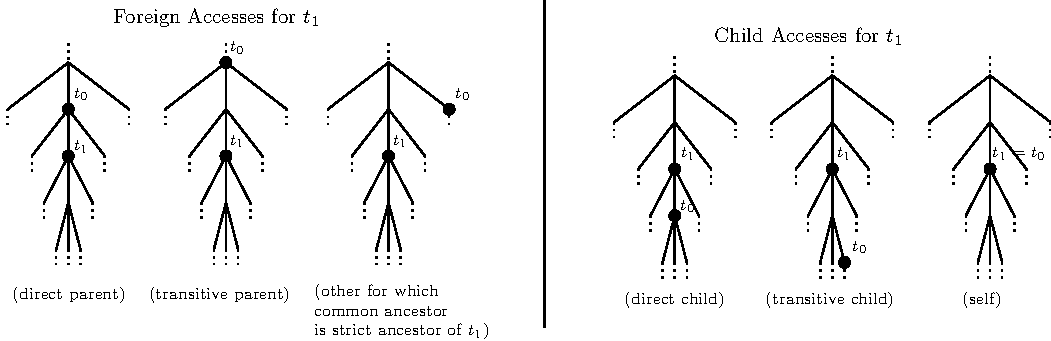
\includegraphics[width=\textwidth]{../figs/accesses-kinds.pdf}
    \caption{Accesses are classified in two categories depending on their relative position
    to the current tag. An access done through a (transitive and inclusive) child tag is a child access.
    An access done through a non-child tag (strict ancestor or non-comparable) is a foreign access.}
    \label{fig:kinds-of-accesses}
\end{figure}


\subsection{Pointer permissions}

\subsubsection{Available permission combinations}

Analysis of the different kinds of pointers leads us to choosing to give pointers
a permission among the following:
\begin{lstlisting}[language=rust]
enum ReadWritePerms {
    Reserved, // Represents a two-phase borrow during its reservation phase
    Active, // Represents an activated (written to) mutable reference
    Frozen, // Represents a shared (immutable) reference
    Disabled, // Represents a dead reference
}
\end{lstlisting}

We choose to introduce \tperm{Reserved} permissions as a way for Tree Borrows to
natively handle two-phase borrows. \tperm{Reserved} does not directly allow write
accesses through this pointer, but it keeps a right to obtain such
write permissions later in the execution.

\subsubsection{two-phase for all borrows}

As we have explained, \tperm{Reserved} represents mutable references with
a two-phase borrow not yet activated.

Rather than limiting this behavior to two-phase borrows only, we choose in Tree
Borrows to make all mutable borrows behave in a uniform way: all mutable references
will wait until their first write access to claim their write permission (become \tperm{Active}),
and will allow shared read-only access in the meantime. If not for this, a lot
of code currently being written would not be accepted, such as some code that
follows the following pattern
\begin{lstlisting}[language=rust]
                               // More generally:
let ptr = vec.as_mut_ptr();  // - some mutable reborrow
if vec.len() > 0 {             // - use base pointer immutably
   do_stuff(ptr)               // - then use the reborrow
}
\end{lstlisting}

A concrete example currently in use in the standard library test suite:
\begin{lstlisting}[language=rust]
let mut x = 2;
let xref = &mut x;
let xraw = &mut *xref as *mut _; // create a mutable reborrow
let xshr = &*xref;
assert_eq!(*xshr, 2); // read-only usage of the base pointer
unsafe {
    *xraw = 4; // usage of the mutable reborrow
}
assert_eq!(x, 4);
\end{lstlisting}

Extending the behavior of two-phase borrows to all mutable borrows also serves
towards our goal of allowing all reorderings of read-only operations: it lets
us exchange reads through mutable (but not used mutably) references with each
other and with reborrows of other mutable references.

\subsubsection{Initialization}

The initial permissions depend of the type of borrow.
Recall from Section \ref{sec:tree-structure} that raw pointers do not receive new permissions and instead
use the same tag and permissions as their parent pointer. This leaves mutable and
shared references for which we must determine an initial permission.

All references allow read accesses initially. This is required
because we perform a fake read access upon reborrowing a reference, and it asserts
that all references are dereferenceable (they are tagged \tcode{dereferenceable}
in LLVM).

In addition, mutable references are allowed to eventually write,
so we initalized them to be \tperm{Reserved}, while shared references are
initialized as \tperm{Frozen}.

\subsection{Updates}
\label{sec:transitions}

We now describe how permissions are updated after an access is performed.
The update process is roughly as follows.

In reaction to an access at \tcode{t0}, traverse the tree. For each \tcode{t1} node of the
tree, if \tcode{t0} is a child of \tcode{t1} then the access is a child access at \tcode{t1}; otherwise
it is a foreign access at \tcode{t1}. Based on the type of access (both child/foreign
and read/write) and some local information, determine the new permissions for the
pointer.

\begin{figure}
    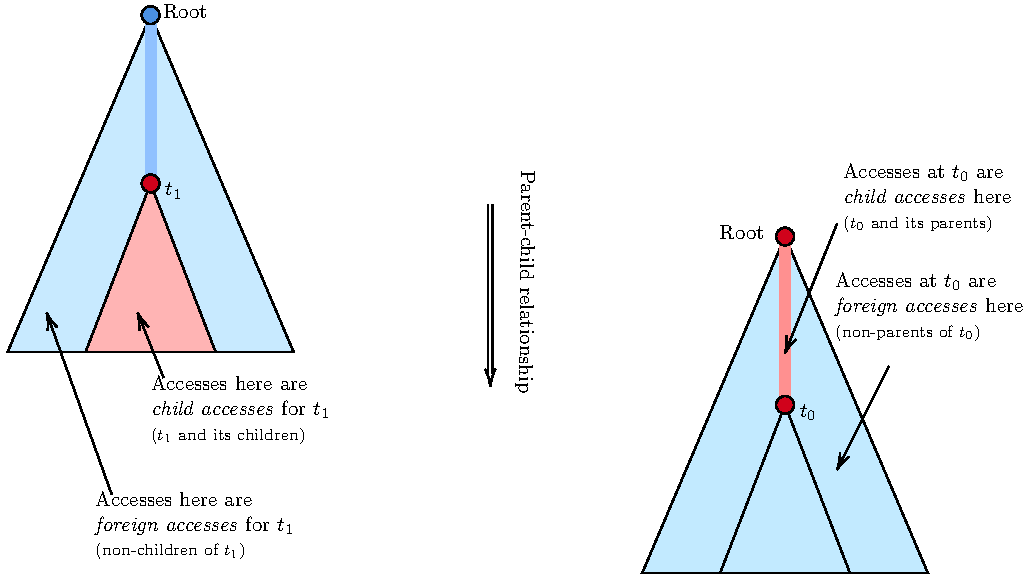
\includegraphics[width=\textwidth]{../figs/child-or-foreign.pdf}
    \caption{Two opposite points of view for the effects of an access.
    Left: how a given tag reacts to accesses at various positions.
    Right: how an access at a given position affects other tags.
    The foreign/child access naming follows the left convention which is easier
    for describing the update of permissions, but the right convention is closer
    to the actual implementation and better explains some optimizations.}
    \label{fig:access-pov}
\end{figure}

\subsubsection{Intuition on effects of accesses}
\label{sec:transitions-basic}

\paragraph*{Child accesses}

If \tperm{Active} is to represent mutable references, then it must allow child writes
as well as child reads. Our interpretation of \tperm{Reserved} as a mutable reference
that is not yet used mutably implies that it much be unaffected by child reads,
but turn into \tperm{Active} on the first child write.

\tperm{Frozen} representing a non-interior-mutable shared reference, it must allow
child reads. As child writes are forbidden on such references, we declare any
child write on a \tperm{Frozen} to be UB.

Any child access is obviously UB on a \tperm{Disabled} since dead references
do not allow accesses.

\paragraph*{Foreign accesses on Frozen}

Since shared references allow shared read access, \tperm{Frozen} must be unaffected
by foreign reads. As shared references on types without interior mutability
assume that no other reference accesses the same data mutably, a \tperm{Frozen} must
become \tperm{Disabled} upon a foreign write.

\paragraph*{Foreign accesses on Active}

Several mutable references cannot coexist with each other or with shared
references, so an \tperm{Active} must not remain \tperm{Active} upon a foreign access.

If another mutable reference is accessed, which corresponds to a foreign write,
then this \tperm{Active} must lose all permissions and become \tperm{Disabled}.

According to the Borrow Checker, an \tperm{Active} loses all permissions on a foreign read:
\begin{lstlisting}[language=rust]
// Example 3.A.1
fn main() {
    let base = &mut 42u64;
    let rmut = &mut *base;
    // base: Reserved
    // |-- rmut: Reserved
    *rmut += 1; // Child write for both base and rmut
    // base: Active
    // |--  rmut: Active
    let _val = *base; // Child read for base; foreign read for rmut
    // base: Active
    // |-- rmut: ???
    let _val = *rmut; // Compilation error
    // According to the Borrow Checker, rmut is no longer readable
}
\end{lstlisting}

However we want Tree Borrows to be suited for proving the validity of reordering
any two adjacent read accesses, which means in particular that reordering two
reads should not introduce new UB.

The following piece of code is accepted:
\begin{lstlisting}[language=rust]
// Example 3.A.2
fn main() {
    let base = &mut 42u64;
    let rmut = &mut *base;
    // base: Reserved
    // |-- rmut: Reserved
    *rmut += 1; // Child write for both base and rmut
    // base: Active
    // |--  rmut: Active
    let _val = *rmut; // Child read for both base and rmut
    // base: Active
    // |-- rmut: Active
    let _val = *base; // Child read for base; foreign read for rmut
    // base: Active
    // |-- rmut: ???
}
\end{lstlisting}
but swapping the two last reads from \textit{Example 3.A.2} would produce \textit{Example 3.A.1} above,
which would be UB if \tperm{Active} were to become \tperm{Disabled} on a foreign read.
We thus choose to make \tperm{Active} become \tperm{Frozen} instead, which means that in
both examples above \tperm{???} should be \tperm{Frozen} and UB occurs in neither.

\paragraph*{Foreign accesses on Reserved}
\label{sec:reserved}

\tperm{Reserved} is a more special case, and its behavior is guided by the following examples
(and more in Appendix \ref{app:reserved}):
\begin{lstlisting}[language=rust]
// Example 3.R.1: Foreign read (standard two-phase borrow example)
// This must not be UB
fn main() {
    let mut x = vec![];
    // x: Reserved
    x.push( // two-phase borrow starts here for x' implicitly reborrowed from x
        // x: Reserved
        // |-- x': Active
        x.len() // Foreign read for x'
        // After this, x' must still be writeable inside Vec::push
        // thus a foreign read must not affect Reserved tags.
    );
}

// Example 3.R.2: Foreign write
// This should be UB
fn main() {
    let mut x = 2;
    let mut xref = &mut x;
    // x: Reserved
    // |-- xref: Reserved
    *x = 3; // Child write for x; foreign write for xref
    // x: Active
    // |-- xref: ???
    *xref = 4; // If this is not UB then we are able to alternate writes
               // between two references that each claim exclusive access.
               // This is bad, so xref must no longer have write permissions.
               // The data has been mutated, so xref also can't claim shared
               // read-only access. Therefore foreign writes must make Reserved
               // turn into Disabled, which causes UB in this example as desired.
    *x = 3;
}

\end{lstlisting}

These suggest that a \tperm{Reserved} should tolerate foreign reads (stays \tperm{Reserved})
but not foreign writes (becomes \tperm{Disabled}). We have already established that
a \tperm{Reserved} allows child reads (stays \tperm{Reserved}) and must be changed
to \tperm{Active} before the first child write.


\subsubsection{Interpretation of transitions using an ordering}

From the conclusions of Section \ref{sec:transitions-basic} we can observe that all transitions follow the order
\tperm{Reserved < Active < Frozen < Disabled}, which corresponds to the permissions
during a ``normal'' lifetime of a mutable reference: it is \tperm{Reserved} upon creation
to accomodate for two-phase borrows, then eventually becomes \tperm{Active} on the first
child write. The next foreign read marks the end of its period of exclusive access
and it can now only be accessed immutably by becoming \tperm{Frozen}. Eventually its
lifetime ends altogether as a different branch claims exclusive access, it
becomes \tperm{Disabled} and will remain so forever.

A possible interpretation of the established transitions would be the following:
\begin{itemize}
    \item in reaction to a child access, the state will advance forward according to \tperm{<} until
        it has obtained the required read/write permissions for the access to be performed
        \begin{itemize}
            \item \tperm{Reserved}, \tperm{Active}, and \tperm{Frozen} already allow reading,
                so a child read does not affect them;
            \item \tperm{Active} also allows writing, so it is unaffected child Write;
            \item \tperm{Reserved} does not directly allow writing, but it can advance to \tperm{Active} to
                obtain the missing permission;
            \item \tperm{Frozen} for a write and \tperm{Disabled} for either a read or a write have no way of
                obtaining the required permissions, since all reachable states are also missing these
                permissions, this produces UB.
        \end{itemize}
    \item in reaction to a foreign access, the state will advance forward according to \tcode{<} until
        it has lost the incompatible read/write permissions
        \begin{itemize}
            \item \tperm{Disabled} having no permissions to lose, it has both many looping transitions and many incoming transitions;
            \item \tperm{Frozen} is the destination for an \tperm{Active} that needs to lose its write permission;
            \item \tperm{Frozen} and \tperm{Reserved} are compatible with a foreign read, hence the loops.
        \end{itemize}
\end{itemize}

In addition, notice that every state that has an incoming transition for any kind of
access also has a loop to itself for the same kind of access. For example a foreign read
access on \tperm{Active} leads to \tperm{Frozen}, which is stable under foreign reads. Similarly
a child write on Reserved leads to \tperm{Active} which is stable under child writes.
In other words, all transitions induced by accesses are idempotent.

This observation is an easy consequence of the ``advance until permissions are compatible''
interpretation of the transitions: once a state has been reached with compatible
permissions, applying the same access again will be a no-op because the state
is obviously already compatible. This idempotency of all accesses opens the door
for optimizations: if the consequences of a certain kind of access have already
been applied to some subtree of the borrow tree, said subtree can be skipped entirely
from the tree traversal if the next access is also of the same kind. This optimization
has been implemented and yields very noticeable improvements (x2 to x5 speedup).


\subsubsection{Protectors}
\label{sec:need-protect}

The compiler optimizations that Tree Borrows should justify include LLVM optimizations,
thus Tree Borrows must not allow violations of assumptions made by LLVM. Among these
assumptions is \tcode{noalias} which specifies to what extent a pointer passed as an
argument to a function aliases with other pointers. In Rust, mutable and shared
references in function arguments are both marked \tcode{noalias}.

\begin{figure}[h]
    \centering
    \begin{minipage}{0.8\textwidth}
        \tcode{noalias}

        This indicates that memory locations accessed via pointer values based on the argument
        are not also accessed, during the execution of the function, via pointer values not based on
        the argument. This guarantee only holds for memory locations that are modified,
        by any means, during the execution of the function.

        --- from the LLVM Language Reference Manual \cite{llvm_langref}
    \end{minipage}
\end{figure}

This can be reworded in language closer to Tree Borrows:

\begin{figure}[h]
    \centering
    \begin{minipage}{0.8\textwidth}
        An access via pointer values based on the argument is a \textbf{child access}.

        An access via pointer values \textbf{not} based on the argument is a \textbf{foreign access}.

        If a tag is marked noalias then during the execution of the function there must
        not be both child and foreign accesses relative to this tag if at least one of them is a write access.
    \end{minipage}
\end{figure}

This makes several pieces of code that would be allowed according to the model so
far be UB according to LLVM. Any code that is UB according to LLVM must also be
UB according to Rust. Examples of such code are shown in Appendix \ref{app:need-protect}.

To remedy this and properly detect this kind of UB, we introduce \textit{Protectors},
named after their Stacked Borrows equivalent.
Upon function entry, we add a Protector to every reference passed as argument, which
is now declared \textit{protected}. Protected pointers behave slightly differently from
unprotected pointers. Protectors are removed when the function returns.

This is implemented by maintaining a \tcode{HashSet} containing call ids of functions that have not yet
returned and their reference arguments, and querying this set on each transition
to know if this tag's permissions should follow the protected or unprotected
version of the transitions. In order to not declare too much UB, we also add
to each state a boolean field \tcode{accessed}, which is initially \tcode{false}
and becomes \tcode{true} on the first child access.

We apply the following rules to pointers that have an active protector
(when the protector is removed upon function exit, these rules no longer apply):

\begin{itemize}
    \item any protected tag becoming \tperm{Disabled} is UB;
    \item \tperm{Reserved} is affected by foreign reads and writes regardless of interior mutability,
        it always becomes \tperm{Frozen} after a foreign read and \tperm{Disabled} after a foreign write;
    \item \tperm{Active} becomes \tperm{Disabled} instead of \tperm{Frozen} on a foreign read.
\end{itemize}

The transitions including protectors can be seen in the state automaton of Figure \ref{fig:state-machine}.

\begin{figure}
    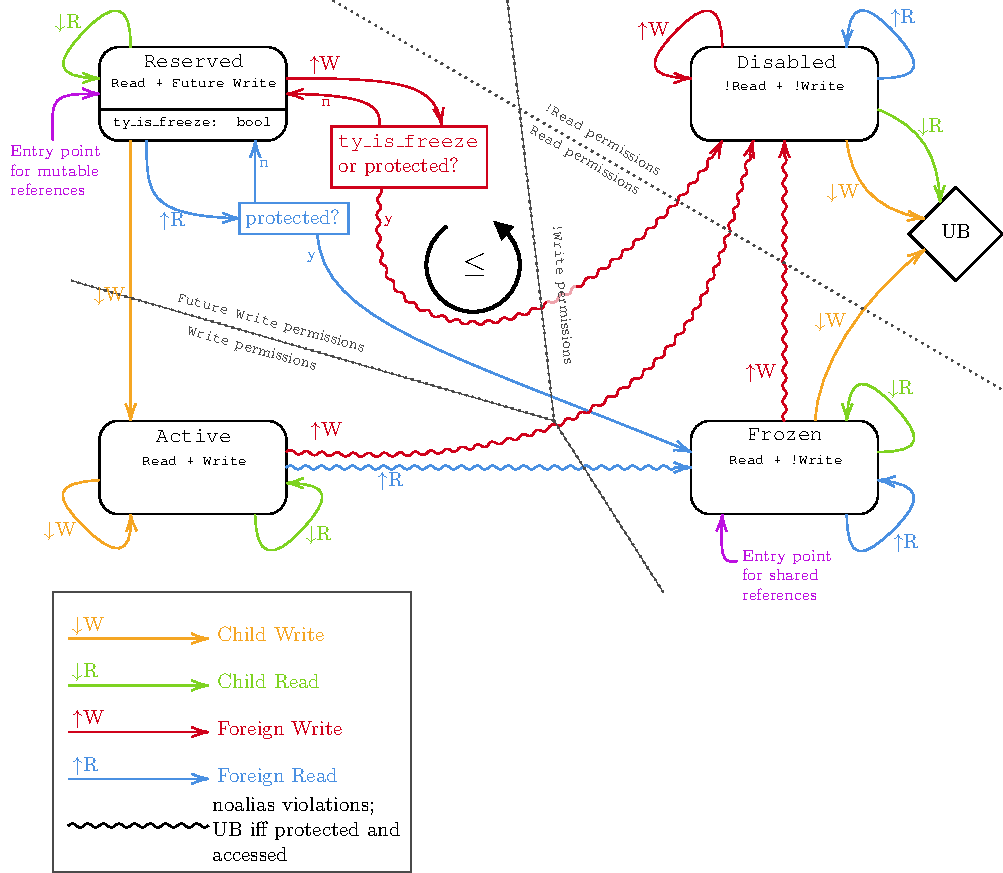
\includegraphics[width=\textwidth]{../figs/state-machine.pdf}
    \caption{State machine for the update of permissions including protectors}
    \label{fig:state-machine}
\end{figure}

\subsubsection{Accesses outside of initial range}

Tree Borrows is capable of handling pointers with unknown size as well as using
a pointer to access data outside of the range it was reborrowed for. One such case is
\begin{lstlisting}[language=rust]
fn access_after_offset() { unsafe {
    let data: [u64; 2] = [0, 1];
    let fst = &mut data[0] as *mut u64; // only reborrowed for [0]
    let snd = fst.add(1); // used on [1], which was not reborrowed
    ptr::swap(fst, snd);
} }
\end{lstlisting}
Here the reborrow for \tcode{fst} only covers \tcode{data[0]}, but \tcode{snd} is then derived from
\tcode{fst} and offset outside of its original range. As we still wish to check
that even for these accesses no aliasing assumptions are violated, we track
permissions even for locations outside of the range of the initial reborrow.

These permissions outside the range can be initialized lazily rather than as soon
as the reborrow occurs, because it is costly to immediately add permissions
on the entire allocation when they will most likely never be actually used by
a child access.

We do not perform a read access on reborrow for locations outside of the range.

\section{Tree Borrows implemented}

All behavior described here was implemented in Miri and is available since
\href{https://github.com/rust-lang/miri/pull/2785}{its recent merge} through
the \texttt{-Zmiri-tree-borrows} flag. Further testing and improvement
of diagnostics are scheduled.

\subsection{Testing the Rust Standard Library}
\label{sec:testing_stdlib}

We used the method described in
\href{https://github.com/rust-lang/miri-test-libstd}{\texttt{github:rust-lang/miri-test-libstd}}
to evaluate on the Standard Library that Tree Borrows does not declare ``too much UB'',
in other words that the code that is currently in use is not considered UB according
to Tree Borrows.

We found two tests that were rejected by Tree Borrows, both were instances of the
following pattern:
\begin{lstlisting}[language=rust]
let mut root = 6u8;        // Base pointer: Active
let mref = &mut root;      // Direct child: Reserved
let ptr = mref as *mut u8; // Uses the same tag as mref
// Write to ptr makes it Active
*ptr = 0;
// Parent read from the point of view of ptr makes it Frozen
assert_eq!(root, 0);
// Attempted write is rejected because Frozen forbids writes
*ptr = 0;
\end{lstlisting}

This pattern was previously accepted by Stacked Borrows, but has now been determined
to be arguably a violation of uniqueness that should not have been accepted in the
first place. It is also easy to patch: the fix (which simply consists of
replacing \tcode{\&mut root as *mut _} with \tcode{addr\_of\_mut!(root)}) was accepted
in \href{https://github.com/rust-lang/rust/pull/107954}{github:rust-lang/rust/pull/107954}.


Other widely used libraries such as \texttt{rand} and \texttt{tokio} already
satisfy the requirements of Tree Borrows, suggesting that most codebases will
need few to no changes if they are to enforce the Tree Borrows semantics.
Checking more thoroughly that this is actually the case is one of the ambitions of our future
work.

\subsection{Performance concerns and optimizations}
\label{sec:perf}

Tree Borrows is slower than Stacked Borrows.
The semantics require that on every access, every tag of the allocation have its
permissions updated on the corresponding range. On allocations with many reborrows
this can easily lead to a naive implementation of Tree Borrows being slower than
Stacked Borrows by an arbitrarily large multiplicative factor.


Fortunately Tree Borrows has access to easy optimizations that allow it to have
an execution time in the same order of magnitude as that of Stacked Borrows on
realistic code samples. We observe in Figure \ref{fig:perf} that in practice the slowdown from Stacked Borrows
to Tree Borrows is mostly less than x2 on benchmarks that are specifically designed
to stress the borrow tracker, and about x1.3 on general tests that don't particularly attempt to
push the borrow tracker to its limits.

Note further that the benchmarks that follow compare a very optimized implementation
of Stacked Borrows with a Tree Borrows implementation that was only optimized up to
the point that it would not waste too much time. Fine-tuning the garbage collector
of unused tags and implementing a cache are likely to improve the performance of
Tree Borrows as they have already done for Stacked Borrows.


\begin{figure}
    \centering
    \begin{tabular}{|l|l|c|c|c|c|}
        \hline
        Project & Test & Runs & SB & TB & Factor \\
        \hline
        \multirow{2}{9em}{Miri}
            & \texttt{slice-get-unchecked} & 5 & 0.44s & 6.87s & {\color{Red}x15.6} \\
            & \texttt{zip-equal} & 5 & 1.66s & 5.68s & {\color{Red}x3.42} \\
            & \texttt{mse} & 5 & 0.45s & 1.48s & {\color{Red}x3.2} \\
            & \texttt{unicode} & 5 & 1.02s & 1.80s & {\color{YellowOrange}x1.76} \\
            & \texttt{serde1} & 5 & 1.52s & 2.65s & {\color{YellowOrange}x1.74} \\
            & \texttt{serde2} & 5 & 3.14s & 5.02s & {\color{YellowOrange}x1.60} \\
            & \texttt{backtraces} & 5 & 3.02s & 4.83s & {\color{YellowOrange}x1.60} \\
        \hline
        \multirow{3}{9em}{Stdlib}
            & \texttt{core} & 1 & 4m31s & 9m15s & {\color{Red}x2.05} \\
            & \texttt{alloc} & 1 & 4m45s & 5m54s & {\color{LimeGreen}x1.24} \\
            & \texttt{std/time} & 1 & 15.1s & 17.5s & {\color{LimeGreen}x1.16} \\
        \hline
        \multirow{1}{9em}{Regex}
            & \texttt{lib} & 1 & 13.3s & 20.6s & {\color{YellowOrange}x1.54} \\
        \multirow{1}{9em}{Hashbrown}
            & \texttt{lib} & 1 & 31.5s & 38.3s & {\color{LimeGreen}x1.21} \\
        \multirow{1}{9em}{Tokio}
            & \texttt{lib} & 1 & 40.7s & 45.3s & {\color{LimeGreen}x1.11} \\
        \multirow{1}{9em}{Rand}
            & \texttt{lib} & 1 & 1m24s & 1m31s & {\color{LimeGreen}x1.08} \\
        \multirow{1}{9em}{Memchr}
            & \texttt{lib} & 1 & 2.1s & 2.2s & {\color{LimeGreen}x1.05} \\
        \hline
    \end{tabular}
    \caption{
        Benchmarks comparing the execution time of variouS test suites
        for Stacked Borrows (SB) or Tree Borrows (TB), including
        Miri's internal tests, standard library tests, and popular crates.
        The increase in computation time is shown to be rarely more than a factor
        \(x1.1\) to \(x1.5\) for real projects, and \(x1.7\) to \(x3\) for worst-case examples.
        Some of these projects use Stacked Borrows as part of their continuous integration
        pipeline, so switching to Tree Borrows is shown to be reasonable in terms of
        additional computational requirement.
        Overall, Miri itself is the most impacted by the performance of Tree Borrows,
        since Tree Borrows performs worse on benchmarks than on real-life examples.
        The Appendix \ref{app:perf} lists the commands and sources
        that were used for each of these benchmarks.
    }
    \label{fig:perf}
\end{figure}

The \texttt{zip-equal} benchmark above was added after we discovered a pathological
case in the test suite of the
\href{https://github.com/hyperium/http/blob/3a2f3e01c01e60b894d1f5b30554013d990010c6/src/header/name.rs#L1685-L1705}{http}
crate. We were able to \href{https://github.com/rust-lang/miri/pull/2865}{fix the issue}
(that came from an improper implementation of the tag garbage collector)
and dramatically improve performance on this specific pattern
(the bug caused a quadratic blowup of the runtime, which we removed).

\subsection{Evaluation of expected backwards-compatibility breakage due to Tree Borrows}

Merely evaluating Tree Borrows on the examples shown in Section \ref{sec:testing_stdlib}
is not sufficient for a complete picture of how Tree Borrows fits in the Rust
ecosystem.

For this, we can rely on the \texttt{crater} tool and the \href{https://crates.io}{crates.io} repository.
\texttt{crates.io} is the main official repository of Rust libraries. Most Rust features
not part of the standard library are published to \texttt{crates.io}, and it even contains some
better-than-stdlib libraries. In its quality of official collection of user-written Rust code,
\texttt{crates.io} is often used to detect bugs in the compiler early: since all code published
to \texttt{crates.io} compiles and passes tests, a simple way to catch backwards incompatibilities
in new versions of the compiler is to run it on the entire codebase of \texttt{crates.io}.
The tool that automates running tests on all of \texttt{crates.io} is called \texttt{crater}.

Miri comes with a fine-tuned \href{https://github.com/saethlin/miri-tools}{fork of \texttt{crater}},
which \href{https://github.com/saethlin}{Ben Kimock} hosts, and using it we obtained the data shown in
\ref{fig:ubcount}.
Using this data we can evaluate in advance how difficult it would be for the Rust ecosystem to
adapt to a new kind of UB: more crates that contain code that Miri considers UB would equate more
compiler breakage in the future if \texttt{rustc} actually implements Miri-based optimizations.

\begin{figure}
    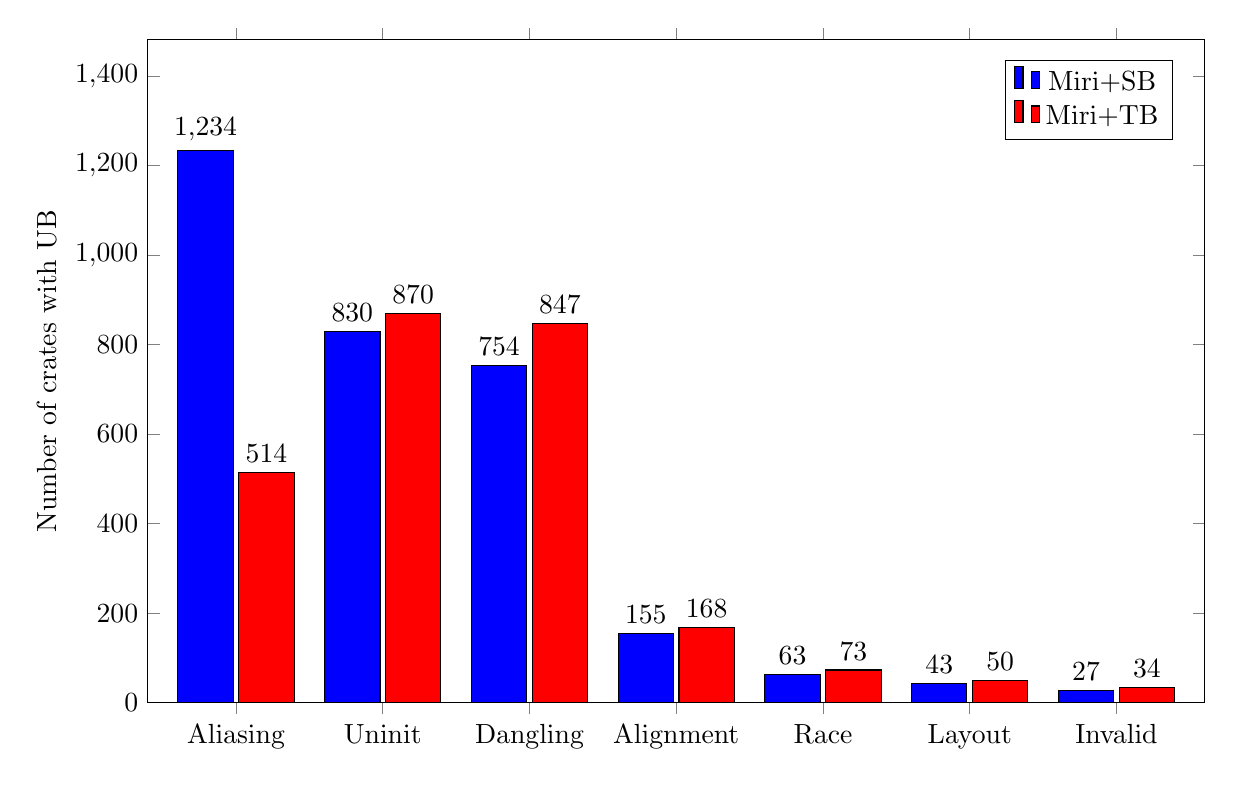
\begin{tikzpicture}
        \begin{axis}[
                ybar,
                ymin=0,
                width=15cm,
                height=10cm,
                bar width=20pt,
                ylabel={Number of crates with UB},
                nodes near coords,
         %      nodes near coords align=below, % places labels inside bars
                symbolic x coords={Aliasing, Uninit, Dangling, Alignment, Race, Layout, Invalid},
                xtick = data,
                enlarge y limits={value=0.2,upper},
                legend pos=north east
            ]
            \addplot[fill=blue] coordinates {(Aliasing, 1234) (Uninit, 830) (Dangling, 754) (Alignment, 155) (Race, 63) (Layout, 43) (Invalid, 27)};
            \addplot[fill=red] coordinates {(Aliasing, 514) (Uninit, 870) (Dangling, 847) (Alignment, 168) (Race, 73) (Layout, 50) (Invalid, 34)};
            \legend{Miri+SB,Miri+TB}
        \end{axis}
    \end{tikzpicture}
    \caption{
        As of May 2023 (when the logs were obtained),
        total number of crates on \href{https://crates.io}{\texttt{crates.io}} (out of 100k)
        whose test suite contains at least one instance of each kind of UB detected by Miri.\\
    }
    \label{fig:ubcount}
\end{figure}

\begin{paragraph}{In Figure \ref{fig:ubcount}, meaning of columns:}
    \begin{itemize}
        \item Aliasing: aliasing UB detected by Stacked Borrows (``Miri+SB'') or Tree Borrows (``Miri+TB'');
        \item Uninit: read of uninitialized memory;
        \item Dangling: dangling or null raw pointer used to create a \tcode{Box} or \tcode{\&mut} (should be non-dangling),
            or dereferencing a dangling pointer;
        \item Alignment: unaligned raw pointer used to create a \tcode{Box} or \tcode{\&mut} (should be aligned),
            or dereferencing an unaligned pointer;
        \item Race: racing accesses to the same data in two threads;
        \item Layout: violations of calling conventions, attempting to deallocate C heap memory which does not match the Rust heap memory layout, zero-size allocation, ...;
        \item Invalid: otherwise invalid value constructed (e.g. a \tcode{bool} that is not \tcode{0} or \tcode{1}, enum discriminant that does not exist, unreadable vtable, ...).
    \end{itemize}
\end{paragraph}

\begin{paragraph}{Methodology}
    We have access to \href{https://miri.saethlin.dev/ub}{miri.saethlin.dev} which records the output of Miri with SB
    on every (100k+) crate on \texttt{crates.io}. We also have an analogue dataset for Miri with TB.

    The dataset consists of a series of records:
    \begin{itemize}
        \item a crate name;
        \item a crate version;
        \item an output among:
            \begin{itemize}
                \item ``Success'', if no error occured;
                \item ``Timeout'', if the crate exceeded its alloted amount of time to run test;
                \item ``Error'', if an environment or runtime error occured (e.g. calling a function not supported by Miri);
                \item ``UB: [list of instances of UB]'', if the crate contains UB in at least one test.
            \end{itemize}
    \end{itemize}
    A crate can contain several instances of UB if different tests each contain UB, but if a single test
    contains several kinds of UB Miri will only be able to report the first one that occurs.
    Each (name, version) pair uniquely identifies a crate.

    In order to reduce noise and ensure a fair comparison between Miri+SB and Miri+TB,
    the dataset was cleaned in the following ways:
    \begin{itemize}
        \item Since the Miri+SB and Miri+TB versions were not run at exactly the same time, we first restrict the
            dataset to only (name, version) pairs that are common across both. This ensures that SB and TB are
            tested on exactly the same code.
        \item Crates that timeout in one but not the other are excluded, since it is possible that UB would have occured
            if the test had ran slightly longer.
        \item Crates that result in a runtime error in one but not the other are also excluded,
            since it may be due to being run with different configurations.
    \end{itemize}

    For the remaining crates, which were all run on both SB and TB and executed all their tests without timing out,
    we count whether at least one of their tests contains an instance of each kind of UB.
    If a crate contains one instance of Aliasing UB and one instance of Uninit UB it will be counted in both columns,
    but if it contains two instances of Aliasing UB then it will only count once towards that number.
    This reduces the impact of crates that have a lot of tests that all contain exactly the same instance of UB
    due to calling a common helper function that contains UB.
\end{paragraph}

\begin{paragraph}{Interpretation}
    Currently all the crates that appear in this count compile withour error and execute correctly
    under the official compiler \texttt{rustc}.
    Miri however is more strict than \texttt{rustc} and considers the amount of crates shown to contain UB of some sort.
    Therefore each column measures in some sense the amount of backwards incompatibility that would come
    from the compiler actually performing the related optimizations.

    In the specific case of Stacked and Tree Borrows, we can see that Tree Borrows causes roughly
    half as many crates to fail than Stacked Borrows, which means that implementing optimizations
    allowed by Tree Borrows would have much less risk of breaking existing code than optimizations
    allowed by Stacked Borrows.

    Anectotal evidence from a handful of popular crates suggests that this effect is even more
    noticeable when authors are actually careful about UB (in other words, Stacked Borrows UB
    has a higher tendency to be hard to avoid even when one is careful about UB):
    in the reported popular crates that contain UB under SB and have actively tried to fix it but failed
    (\texttt{tokio}, \texttt{pyo3}, \texttt{rkyv}, \texttt{eyre}, \texttt{ndarray}, \texttt{arrayvec},
    \texttt{slotmap}, \texttt{nalgebra}, \texttt{json}), all of them were found to be free of UB under TB.
\end{paragraph}

\begin{paragraph}{UB Shadowing}
    The reader may be surprised to see that while Miri+TB has much less Aliasing UB than Miri+SB,
    it has slightly more of every other kind of UB. There is a very simple explanation for that,
    simply by virtue of how Miri reports UB.

    In a given test, Miri executes the code until it detects UB, and when it does it aborts the test
    and outputs an error message. Therefore if a single test contains several instances of UB
    Miri will only report the first one. Some errors related to e.g. accessing uninitialized memory
    happen by simple coincidence to also be aliasing errors, or to be preceded chronologically by
    aliasing errors. This occurs frequently for at least the following reasons: (a) programmers
    who are not careful about uninitialized memory probably tend to also not be careful about aliasing,
    and (b) programs that manipulate uninitialized memory definitely use \texttt{unsafe} code and probably
    use that memory in nontrivial ways, which makes aliasing errors more likely.

    There is thus an increased likelyhood in a test for which Miri+SB reports Aliasing UB
    that it also contains Uninit UB, but the Uninit UB is ``shadowed'' by the Aliasing UB that occurs
    first. If Miri+TB no longer reports Aliasing UB for that specific test, it still contains Uninit UB.
    Thus with the move from Miri+SB to Miri+TB, the following happens:
    \begin{itemize}
        \item some tests that contain exclusively SB Aliasing UB are removed from the count entirely,
        \item some tests that contain SB Aliasing UB and also another kind of UB are recategorized under
            only said other kind.
    \end{itemize}
    This accounts for the entirety of the increased counts of every kind of UB other than Aliasing.

    By being more permissive, Tree Borrows thus allows some tests that were
    thought to contain Aliasing UB to be more accurately recategorized under other kinds of UB.

    The significance of this should not be underestimated: not only does Miri+TB still contain much fewer
    instances of UB than Miri+SB overall, it may also encourage more crate authors to actually fix the remaining UB.
    Indeed SB has a reputation for being too strict, and for years now it has been known that SB as it currently
    is would not become the standard. Programmers that encounter an SB error message may thus tend to automatically
    dismiss it as a problem for later, or something that will never become the standard anyway.
    On the other hand it is much more well-known that uninitialized memory could be dangerous immediately,
    so an Aliasing+Uninit bug is more likely to be fixed if it is classified as Uninit than as Aliasing.
\end{paragraph}

\begin{paragraph}{Limitations}
    There is an obvious bias in evaluating TB only on published crates: this disregards a lot of
    Rust code that is being written, including most notably (a) closed-source libraries or big
    projects not published to \texttt{crates.io}, and (b) code written by beginners who do not
    yet have the knowledge or confidence to publish to \texttt{crates.io}.
    This bias is likely of minimal consequence, since TB only has an impact on code that uses
    \texttt{unsafe} Rust, which both of the above categories tend to avoid (beginners do
    not use \texttt{unsafe} until they have more experience, and large projects still tend out
    of habit to publish small logical chunks of the parts of their codebase that require \texttt{unsafe}
    as independent libraries).

    A more actionable concern is over the quality of the data we have access to.
    Out of the 121,164 crates currently published, there are 105,904 that were executed under both
    Miri+SB and Miri+TB with the same version (during the few weeks that separated the executions
    of Miri+SB and Miri+TB many crates rolled out a new version that was only tested on Miri+TB).
    Of them 32,585 must be eliminated because both Miri+SB and Miri+TB timeout or error,
    but a further 20,410 were removed because only one of Miri+SB or Miri+TB timed out.
    This leaves a usable dataset of 52,909 points, which wastes about a third of what could be
    available if we executed Miri+SB and Miri+TB closer in time to each other and paid closer
    attention to them having otherwise identical configurations.

    The tool that lets us perform these measurements is costly to run (it takes several days to
    fully execute and generates upwards of 50Gb of logs) and currently under maintenance,
    but if an opportunity arises to run it once more, we should make sure that fewer data points
    are wasted due to timeouts and environment errors.
\end{paragraph}

\subsection{Experiments about \tcode{Unique}}

The \tcode{core} library defines a wrapper type around a pointer, \tcode{ptr::Unique<T>} that -- according to
its own \href{https://doc.rust-lang.org/src/core/ptr/unique.rs.html#11}{documentation} --
is supposed to logically ``behaves as if it were an instance of \tcode{T}'',
including having ``the kind of strong aliasing guarantees an instance of \tcode{T} can expect''.

We have naturally decided to experiment to see if TB is suited to specifying the semantics
of \tcode{Unique}, and have added to Miri
\href{https://github.com/rust-lang/miri/pull/2936}{experimental support for treating \texttt{Unique}
the same way as a mutable pointer} (in contrast to the default which is to ignore it
and not reborrow the inner pointer). \\

We expected to face difficulties during this experiment, because \tcode{Unique} is used internally
inside \tcode{Vec} (the standard library dynamically-sized array), and a lot of code that uses
\tcode{Vec} e.g. to implement an arena allocator could run into aliasing issues.

The current version of this experiment was found to be unsound when we discovered a piece
of safe code that triggers UB under this experimental behavior, so in their current form
these semantics of \tcode{Unique} cannot be stabilized. Unsurprisingly, this example
involves tricky interactions between the different components of a \tcode{Vec<Cell<Unique<T>>>},
that is it combines into one all the difficult cases of interior mutability and uniqueness.

We have ideas on how this could be circumvented (for example \tcode{Unique} could have
special semantics only when it is protected, or only when it is not also interior
mutable), but none of them were tested thoroughly enough to become the default in Miri,
so the current state of experiments around \tcode{Unique} is to be turned off by default.
Future work may explore further the implications and constraints of enforcing uniqueness
of \tcode{Unique}.

\section{Proving optimizations}

\subsection{Intuition}

We show a sketch of how to use Tree Borrows to prove some reordering-based optimization.
\begin{lstlisting}[language=rust]
fn example2_unopt(x: &u64) -> u64 {
    let val = *x;
    g(); // arbitrary (possibly unsafe) unknown code modeled by a function call
    val
}

fn example2_opt(x: &u64) -> u64 {
    g();
    *x // This optimization is a read/call reordering + value propagation
}
\end{lstlisting}

For the above reordering to be valid, the following needs to hold.
For any definition of \tcode{g}, for any context \(C\), if \(C[\texttt{example2\_unopt}]\)
does not exhibit UB then \(C[\texttt{example2\_opt}]\) also does not exhibit UB.
We call \(C[\texttt{example2\_unopt}]\) the source, and \(C[\texttt{example2\_opt}]\)
the target.

Proof sketch: it is sufficient to prove that if \tcode{example2\_unopt} and \tcode{example2\_opt}
are executed with the same memory state and initial borrow tree
for which \tcode{example2\_unopt} does not trigger UB then
\begin{itemize}
    \item \tcode{example2\_opt} does not trigger UB, and
    \item they both modify the memory in the same way, and
    \item they return the same value, and
    \item they result in the same final borrow tree.
\end{itemize}

Indeed if neither triggers UB immediately and they result in the same memory
state and borrow tree then the two versions of the function will be indistinguishable
without UB in the source.

We mark the following notable points of the code:
\begin{lstlisting}[language=rust]
fn example2_unopt(x: &u64) -> u64 {
    // s0
    let val = *x;
    // s1
    g();
    // s2
    val
    // s3
}

fn example2_opt(x: &u64) -> u64 {
    // t0
    g();
    // t1
    *x
    // t3
}
\end{lstlisting}
and denote \(T(x)\) and \(M(x)\) the tree and memory at the execution point \(x\).

Let \(l\) the location that \tcode{x} points to: \(M(s_0)[l]\) is the value
of \tcode{*x} at \(s_0\).

We first show that \tcode{g} must not perform a write to \(l\). We have created
a fresh tag \(p_x\) for \tcode{x} and no child tag of \(p_x\) has been passed
to \tcode{g}, thus any access that occurs during \tcode{g} is a foreign access
for \(p_x\). Since \(p_x\) is protected, any foreign write would be UB, thus
\tcode{g} can be assumed not to perform any write access to \(l\).
Therefore the value at \(l\) in unchanged during the execution of \tcode{g} in
the source. This proves that both functions return the same value.

Assuming \(M(s_0) = M(t_0)\) since the two functions are to be executed in the
same context, and since no write occurs at all between \(s_0\) and \(s_1\)
we thus obtain \(M(s_1) = M(t_0)\). In the source and the target the whole memory
is identical when \tcode{g} is called, thus \tcode{g} executes in the same way
in both. Since no memory modification occurs between \(s_2\) and \(s_3\) or between
\(t_1\) and \(t_3\), we obtain that \(M(s_3) = M(t_3)\).

What remains is to show that the source and target result in the same
borrow tree and that the target does not have UB. Since \(T(t_0)\) refines
\(T(s_1)\), no UB occurs in the target during the execution of \tcode{g}.
We then examine what happens to all borrows for the location:
\begin{itemize}
    \item \(p_x\) in the source is subjected to a child read then zero or more
        child reads during \tcode{g}. It does not matter the order, the final
        permission of \(p_x\) will be the same in the target, i.e. \tperm{Frozen};
    \item there are no children of \(p_x\);
    \item non-children of \(p_x\) that already existed before the execution
        of the function are subjected in the target to the operations in \tcode{g}
        then a read of \(t_x\) instead of the opposite in the source. We easily
        check that in the state machine all transitions induced by read accesses
        (both child and foreign) commute with each other and thus the final
        permissions are the same in the source and in the target.
    \item non-children of \(p_x\) that were created during the execution of \tcode{g}
        are not protected when \tcode{*x} is read in the target and they are not
        \tperm{Active} because creating an \tperm{Active} requires a write.
        The read is thus a no-op.
\end{itemize}

We have thus shown that in the absence of UB in the source,
\(T(s_0) = T(t_0) \Longrightarrow T(s_3) = T(t_3)\) and
thus the source and target have the same behavior, and moving a read access
down across unknown code within a function is a valid optimization.

\subsection{Formal proofs of disjointness}

After formalizing in Coq the rules of Tree Borrows (Coq code can be found at\\
\href{https://gitlab.mpi-sws.org/neven/simuliris/-/tree/master/theories/tree_borrows}{\texttt{gitlab.mpi-sws.org/neven/simuliris}},
explanations also in \ref{app:formalization})
, we were able to prove directly against the operational semantics that
\begin{itemize}
    \item if two accesses occur through unrelated pointers without triggering UB and at least one of
        them is a write then the ranges of memory for these accesses must be disjoint,
    \item if two consecutive accesses occur on disjoint ranges of memory then they can be permuted
        and the final state is identical to the one before the permutation,
    \item two adjacent read accesses can always be permuted.
\end{itemize}

This proves that Tree Borrows satisfies the minimum requirements of justifying LLVM
optimizations, since in all cases where LLVM would assume that two pointers point
to disjoint ranges of memory, said disjointness is a consequence of the absence of
Tree Borrows UB. And in all cases where LLVM could reorder accesses, the model
assigns the same final state to both orderings.


\subsection{Invariants}

Another method of proving optimizations is to establish some invariants that
\begin{itemize}
    \item hold on an access through a pointer \tcode{x},
    \item are preserved by every (possibly restricted to foreign) access for \tcode{x},
    \item allow accessing \tcode{x} again with guarantees on its value.
\end{itemize}

This is the same method used in \cite{simuliris} to prove Stacked Borrows reorderings,
and this is the kind of reasoning that it allows: consider the property
\[F(\text{\tcode{x}}, s) := \text{\tcode{x.permission}} \ne \text{\tcode{Disabled}} \Rightarrow \text{\tcode{x.permission = Frozen}} \wedge \text{\tcode{x.value}} = s\]
and observe that
\begin{itemize}
    \item \(F(\text{\tcode{x}, s})\) holds when a read through \tcode{x} a shared reference succeeds and returns \tcode{s},
    \item \(F(\text{\tcode{x}, s})\) is preserved by every access that does not trigger UB:
        \begin{itemize}
            \item a foreign or child read changes neither the permission nor the value,
            \item a child write triggers UB because writing through \tcode{Frozen} is forbidden,
            \item a foreign write makes the precondition false by disabling \tcode{x}.
        \end{itemize}
\end{itemize}
Now consider that if \(F(\text{\tcode{x}}, s)\) holds while the program executes a child read,
then by assuming that the child read does not trigger UB we get \(\text{\tcode{x.permission}} \ne \text{\tcode{Disabled}}\),
and this implies \(\text{\tcode{x.value}} = s\).

Thus with this simple invariant we are able to prove that reads through the same shared reference
must always return the same value, which is instrumental in proving that they can be reordered with other
operations.


This technique -- provided we are able to find sufficiently strong invariants -- should in
theory allow us to prove the following reorderings:
\begin{itemize}
    \item grouping reads (reorder \tcode{read(x); call(); read(x)} into \tcode{read(x); read(x); call()}),
    \item delaying reads while a protector is active (reorder \tcode{read(x); call()} into \tcode{call(); read(x)}),
    \item grouping writes while a protector is active (reorder \tcode{write(x); call(); write(x)} into \tcode{write(x); read(x); write()}),
    \item delaying writes while a protector is active (reorder \tcode{write(x); call()} into \tcode{call(); write(x)}),
\end{itemize}
which constitute almost all of the optimizations that were proven for Stacked Borrows using the same method.

We have unfortunately encountered an obstacle in trying to complete these proofs: some of them require
reasoning about data races, which we do not have the machinery for.
When we try to reorder \tcode{read(x); call(); read(x)} into \tcode{read(x); read(x); call()}, we need
to prove that no access races with the second read in the target (after reordering). This intuitively
just amounts to ``if there was an access that raced with the second read in the target, then because
there is no thread synchronization between the two read accesses there would already have been a race
condition with the first read from the source (before reordering): by assuming that the source
contains no data race UB we get that neither does the target.''

Expressing this formally requires deep changes to the model, that Stacked Borrows has cleverly avoided
by using a trick that reads that would cause UB instead succeed and return a poison value that only
triggers UB when actually used. This trick is no longer sufficient in Tree Borrows, and so we would
need a lot more work to prove the same properties. This is the topic of ongoing work.


\section{Conclusion}

I believe that although Tree Borrows is still not precise enough to serve as an official standard,
we have made great progress towards stabilizing a model for pointer aliasing in Rust that avoids
the known shortcomings of previous attempts. Feedback from the community suggests that most do indeed
consider Tree Borrows more intuitive than Stacked Borrows, experimental evidence confirms that
Tree Borrows is permissive enough not to be a major concern for backwards compatibility if it is
to ever be enforced, and we have formal proofs that Tree Borrows does permit the optimizations
that it set out to enable.

There is still much room for future work related to
\begin{itemize}
    \item a more thorough look at how interior mutability should be handled consistently,
    \item whether \tcode{core::ptr::Unique} can be given precise semantics that do not restrict
        its flexibility too much,
    \item if spurious writes can ever be allowed without invalidating existing libraries,
    \item performance improvements and fine-tuning,
    \item whether reasonings on data races can be bypassed.
\end{itemize}

% ------------------------------------------------------------------------------

\newpage

\bibliography{literature}


\appendix

\newpage
\section{Benchmarks for Section \ref{sec:perf}}
\label{app:perf}

The benchmarks from Figure \ref{fig:perf} were executed with the following commands.
By default Stacked Borrows is used, and Tree Borrows is selected by appending
\texttt{-Zmiri-tree-borrows} to the list of \texttt{MIRIFLAGS}.

\begin{itemize}
    \item Miri\\
        These benchmarks are designed specifically to exhibit pathological behaviors of
        Stacked Borrows. It happens that many of these are also pathological cases for Tree Borrows,
        in particular very narrow trees (stack-like, obtained by chaining many reborrows)
        and very wide trees (obtained by reborrowing many times from the same pointer).
        It is within expectations that Tree Borrows would perform worse in comparison
        to Stacked Borrows on these tests than on other tests.
        \begin{description}
            \item[Source] \href{https://github.com/rust-lang/miri}{\texttt{github:rust-lang/miri}}
            \item[Command] \texttt{MIRIFLAGS="" ./miri bench}
        \end{description}
    \item Miri-test-libstd\\
        These tests constitute the OS-independent test suites of the Rust standard library. They
        are already used to detect regressions in either Miri or Rustc, but this check currently
        uses Stacked Borrows and not Tree Borrows.
        \begin{description}
            \item[Source] \href{https://github.com/rust-lang/miri-test-libstd}{\texttt{github:rust-lang/miri-test-libstd}}
            \item[Command] \texttt{MIRIFLAGS="" ./run-test.sh core --lib --tests}
            \item[Command] \texttt{MIRIFLAGS="" ./run-test.sh alloc --lib --tests}
            \item[Command] \texttt{MIRIFLAGS="-Zmiri-disable-isolation"}\\
                \texttt{./run-test.sh std --lib --tests -- time::}
        \end{description}
    \item Tokio\\
        This crate is a framework for writing asynchronous code. Since it uses \tcode{unsafe} and
        parallelism in nontrivial ways, detecting UB is important.
        \begin{description}
            \item[Source] \href{https://github.com/tokio-rs/tokio}{\texttt{github:tokio-rs/tokio}}
            \item[Command] \texttt{MIRIFLAGS="-Zmiri-disable-isolation -Zmiri-tag-raw-pointers"} \\
                \texttt{cargo +nightly miri test --features full --lib}
        \end{description}
    \item Rand\\
        This crate is the most widely used crate for random number generation.
        Rand is historically relevant to one of the main
        issues \cite{issue_raw_range_strict}
        of Stacked Borrows' handling of out-of-range raw pointers.
        \begin{description}
            \item[Source] \href{https://github.com/rust-random/rand}{\texttt{github:rust-random/rand}}
            \item[Command] \texttt{MIRIFLAGS="" cargo +nightly miri test --lib}
        \end{description}
    \item Hashbrown\\
        This crate implements a high-performance hash map, which naturally involves aliasing and \tcode{unsafe}.
        \begin{description}
            \item[Source] \href{https://github.com/rust-lang/hashbrown}{\texttt{github:rust-lang/hashbrown}}
            \item[Command] \texttt{MIRIFLAGS="" cargo +nightly miri test --lib}
        \end{description}
    \item Regex\\
        As the name suggests this is a crate for parsing, compiling, and executing regular expressions.
        The test \texttt{encode\_decode} is ignored because it takes too long for Miri to execute.
        \begin{description}
            \item[Source] \href{https://github.com/rust-lang/regex}{\texttt{github:rust-lang/regex}}
            \item[Command] \texttt{MIRIFLAGS="" cargo +nightly miri test --lib -- --skip encode\_decode}
        \end{description}
    \item Memchr\\
        High-performance implementation of standard string search primitives.
        Historically had a conflict with Stacked Borrows as stated in
        \href{https://github.com/BurntSushi/memchr/issues/58}{Issue \#58}
        \begin{description}
            \item[Source] \href{https://github.com/BurntSushi/memchr}{github:BurntSushi/memchr}
            \item[Command] \texttt{MIRIFLAGS="" cargo +nightly miri test}
        \end{description}
\end{itemize}

\newpage
\section{Requirements of protectors}
\label{app:need-protect}

To show why protectors are needed and why they require some alternative
transitions, we show here examples of programs that are UB according to LLVM,
but would not be UB according to Tree Borrows \textbf{if protected pointers behaved identically to unprotected pointers}.
This is a continuation of the example shown in Section \ref{sec:need-protect}.

\subsection{Increased requirements of \tperm{Reserved}}

The following program justifies that after a foreign read has occured, \tperm{Reserved} must no longer allow
foreign reads. Indeed if \tperm{Reserved} is unaffected by foreign reads then it allows a foreign read
followed by a child write. We model this by making \tperm{Reserved} become \tperm{Frozen} on a foreign read,
which means that the next attempted child write would correctly be UB.

For the same reason \tperm{Reserved} must not stay \tperm{Reserved} after a foreign write even
if it has interior mutability: we declare that under a foreign write, \tperm{Reserved} becomes
\tperm{Disabled} regardless of interior mutability which means that the next attempted child read or write would be UB.

\begin{lstlisting}[language=rust]
fn main() {
    let data = &mut 42u64;
    let y = data as *const u64;
    let x = &mut *data;
    foreign_read_before_write(x, y);
    fn foreign_read_before_write(x: &mut u64, y: *const u64) {
        // x: Reserved [noalias]
        let _ = unsafe { *y }; // Foreign read for x
        // x: Reserved [noalias]
        *x += 1; // Child write for x
        // /!\ Combined with the previous foreign read this is a noalias violation
        // x: Active [noalias]
        // -- UB must occur before this point --
        // (Without protectors no UB occurs)
    }
}
\end{lstlisting}


\subsection{Loss of read permissions}

A \tperm{Frozen} pointer becoming \tperm{Disabled} is a symptom that a foreign write occured after
a child read. Indeed a foreign write is only possible cause of the transition in question.
If the location was also accessed through any child access, then these two accesses violate
\tcode{noalias}, thus a transition \tperm{Frozen -> Disabled} should be UB on any accessed location.
The same remark applies to a \tperm{Reserved} or \tperm{Active} becoming \tperm{Disabled}.

\begin{lstlisting}[language=rust]
fn main() {
    let data = &mut 42u64;
    let y = data as *mut u64;
    let x = &*data;
    read_before_foreign_write(x, y);
    fn read_before_foreign_write(x: &u64, y: *mut u64) {
        // x: Frozen [noalias]
        let _ = *x; // Child read for x
        // x: Frozen [noalias]
        unsafe { *y += 1; } // Foreign write for x
        // /!\ Combined with the previous child read this is a noalias violation
        // x: Disabled [noalias]
        // -- UB must occur before this point --
        // (Without protectors no UB occurs)
    }
}
\end{lstlisting}


\subsection{Loss of write permissions}

An \tperm{Active} pointer becoming \tperm{Frozen} indicates the presence of a child write
(requirement for the existence of an \tperm{Active}) and a foreign write (only possible cause
of the transition). These two accesses violate \tcode{noalias}, thus a transition \tperm{Active -> Frozen}
should be UB.

\begin{lstlisting}[language=rust]
fn main() {
    let data = &mut 42u64;
    let y = data as *const u64;
    let x = &mut *data;
    write_before_foreign_read(x, y);
    fn write_before_foreign_read(x: &mut u64, y: *const u64) {
        // x: Reserved [noalias]
        *x += 1; // Child write for x
        // x: Active [noalias]
        let _ = unsafe { *y }; // Foreign read for x
        // /!\ Combined with the previous child write this is a noalias violation
        // x: Frozen [noalias]
        // -- UB must occur before this point --
        // (Without protectors no UB occurs)
    }
}
\end{lstlisting}

\newpage
\section{Behavior of \tperm{Reserved}}
\label{app:reserved}

In addition to the examples shown in Paragraph \ref{sec:reserved}, about
\tperm{Reserved}, some details of the behavior are guided by the observations
that follow.

This pattern is used frequently in the standard library test suite,
it would preferably not be UB.
It consists of a read access through a raw pointer between the creation
and access of a mutable reference, and it illustrates why Tree Borrows
uses the \tperm{Reserved} permission for all mutable references and not
just for two-phase borrows.
\begin{lstlisting}[language=rust]
// Example: Foreign read outside two-phase borrow
// This should not be UB.
fn main() {
    let mut x = 2;
    let xref = &mut x;
    let xraw = &mut *xref as *mut _;
    let xshr = &*xref;
    // x: Reserved
    // |-- xref: Reserved
    //     |-- xraw: Reserved
    //     |-- xshr: Frozen
    assert_eq!(*xshr, 2); // This is a foreign read for xref and xraw
    unsafe { *xraw = 4; } // This is a child write for xref and xraw
                          // meaning it must still be writeable at this point,
                          // therefore the above foreign read must not have turned
                          // them Frozen.
    assert_eq!(x, 4);
}
\end{lstlisting}


This second pattern shows that mutable references that involve interior mutability
must be exempt from the rule that a \tperm{Reserved} is disabled upon a foreign
write. This is safe code, it must absolutely not be UB.
\begin{lstlisting}[language=rust]
// Example: Foreign write with interior mutability
// This must not be UB
fn main() {
    use std::cell::Cell;
    trait Thing: Sized {
        fn do_the_thing(&mut self, _s: ());
    }

    let mut x = Cell::new(1);
    // x: Reserved
    x.do_the_thing({
        // A two-phase borrow starts here for x' implicitly reborrowed from x
        // x: Reserved
        // |-- x': Reserved
        x.set(3) // This is a foreign write for x'
        // x: Active
        // |-- x': ???
    })
    impl<T> Thing for Cell<T> {
        fn do_the_thing(&mut self, _s: ()) {
            // Function call starts, x' is implicitly reborrowed into x''
            // x: Active
            // |-- x': ???
            //     |-- x'': Reserved
            self.set(5): // x' must be readable and writeable
                         // This is a child write for x', which means
                         // that x' is now Active and was not previously Disabled
                         // or Frozen. Therefore x' was previously still Reserved,
                         // even though it was subjected to a foreign write.
        }
    }
}
\end{lstlisting}



\newpage
\section{Summary of the model}

Below is a summary of the points established in \ref{sec:tree_additions} and \ref{sec:transitions}
as a full description of Tree Borrows.

\paragraph*{When creating a new pointer \tcode{z} from an existing \tcode{y}}
\begin{itemize}
    \item if \tcode{z} is a \tcode{Unpin} mutable reference
        \begin{itemize}
            \item perform the effects of a read access through \tcode{y} on the reborrowed range
            \item add a new child of \tcode{y} in the tree
            \item give it the permissions \tperm{Reserved}
                (immediately on the reborrowed range, lazily on the rest of the allocation)
            \item keep track of whether it has interior mutability or not
        \end{itemize}
    \item if \tcode{z} is a non-interior-mutable shared reference
        \begin{itemize}
            \item perform the effects of a read access through \tcode{y} on the reborrowed range
            \item add a new child of \tcode{y} in the tree
            \item give it the permissions \tperm{Frozen}
                (immediately on the reborrowed range, lazily on the rest of the allocation)
        \end{itemize}
    \item otherwise give \tcode{z} the same tag as \tcode{y}, they are indistinguishable from now on
\end{itemize}

\paragraph*{When reading through a pointer \tcode{y}}
\begin{itemize}
    \item for all ancestors \tcode{x} of \tcode{y} (including \tcode{y}), this is a child read
        \begin{itemize}
            \item assert that \tcode{x} has read permissions (i.e. is \tperm{Frozen} or \tperm{Reserved} or \tperm{Active})
            \item otherwise (if \tcode{x} is \tperm{Disabled}) this is UB
        \end{itemize}
    \item for all non-ancestors \tcode{z} of \tcode{y} (excluding \tcode{y}), this is a foreign read
        \begin{itemize}
            \item turn \tperm{Active} into \tperm{Frozen}; this is UB if \tcode{z} is protected
            \item if \tcode{z} is protected, turn \tperm{Reserved} into \tperm{Frozen}
        \end{itemize}
\end{itemize}

\paragraph*{When writing through a pointer \tcode{y}}
\begin{itemize}
    \item for all ancestors \tcode{x} of \tcode{y} (including \tcode{y}), this is a child write
        \begin{itemize}
            \item turn \tperm{Reserved} into \tperm{Active}
            \item it is UB to encounter either \tperm{Disabled} or \tperm{Frozen}
        \end{itemize}
    \item for all non-ancestors \tcode{z} of \tcode{y} (excluding \tcode{y}), this is a foreign write
        \begin{itemize}
            \item if \tcode{z} is protected this is always UB; otherwise
            \item if \tcode{z} is \tperm{Reserved} and has interior mutability it is unchanged; otherwise
            \item turn all of \tperm{Reserved}, \tperm{Active}, and \tperm{Frozen} into \tperm{Disabled}.
        \end{itemize}
\end{itemize}




\newpage
\section{Formalization}
\label{app:formalization}

We formalize Tree Borrows in Coq using some \texttt{Iris} and \texttt{stdpp} dependencies,
of which the following is a rephrasing.
See  \href{https://gitlab.mpi-sws.org/neven/simuliris/-/tree/master/theories/tree_borrows}{\texttt{gitlab.mpi-sws.org/neven/simuliris}},
for the actual formulation.

% preliminaties (accesses, ...)

\newcommand{\kw}[1]{%
    \csdef{#1}{\textsc{#1}}%
}
\newcommand{\field}[1]{%
    \csdef{#1}{\texttt{#1}}%
}
\newcommand{\fn}[1]{%
    \csdef{#1}{\textit{#1}}%
}

\kw{Loc}
\kw{AccessKind} \kw{Read} \kw{Write}
\kw{AccessRel} \kw{Child} \kw{Foreign}
\kw{Access}
\kw{Tag}
\kw{Permission} \kw{Reserved} \kw{ResIntMut} \kw{Active} \kw{Frozen} \kw{Disabled}
\kw{LazyPermission}
\kw{CallID}
\kw{ProtectorKind} \kw{Strong} \kw{Weak}
\kw{Protector} \field{kind} \field{call}
\kw{Item} \field{tg} \field{prot} \field{initperm} \field{perms}
\kw{Tree}
\kw{Set}
\fn{insert} \fn{map} \fn{unique} \fn{related} \fn{fresh}
\fn{access}
\kw{Event} \kw{AccessEvt} \kw{InitCallEvt} \kw{EndCallEvt} \kw{RetagEvt}
\field{locs} \field{cid} \field{parent}
\fn{disjoint}

\newcommand{\finmap}{\xrightarrow{fin}}
\newcommand{\borstep}[1]{\xrightarrow[#1]{}}
\newcommand{\borseq}[2]{\xrightarrow[#1]{#2}}

\subsection{Model encoding}

We use a memory model with locations of type \(\Loc := \mathbb{N} \times \mathbb{Z}\)
(separated by allocation).

Define the different types of accesses as
\begin{align*}
    \AccessKind :=& \set{\Read, \Write} \\
    \AccessRel :=& \set{\Child, \Foreign} \\
    \Access :=& \AccessKind \times \AccessRel
\end{align*}

And the permissions they act upon:
\begin{align*}
    \Tag :=& \mathbb{N} \\
    \CallID :=& \mathbb{N} \\
    \ProtectorKind :=& \set{\Strong, \Weak} \\
    \Protector := &\{\kind:\ProtectorKind \\
                  &| \call:\CallID \\
                  &\} \\
    \Permission &:= \set{\Reserved, \ResIntMut, \Active, \Frozen, \Disabled} \\
    \LazyPermission &:= \Permission \times \text{bool} \\
    \Item := &\{\tg:\Tag \\
             &| \prot:\Protector? \\
             &| \initperm:\Permission \\
             &| \perms:(\Loc \finmap \LazyPermission) \\
             &\}
\end{align*}

We define \(\Tree\) as the set of finite trees with nodes in \(\Item\),
on which the operations \(\insert : \Tag \to \Item \to \Tree \to \Tree\)
(inserts the item as a child of every node with a matching tag) and
\(\map : (\Item \to \Item) \to \Tree \to \Tree\) (applies the function
to every node of the tree) are defined and satisfy the properties you would
expect, such as
\[\forall i\in\Item, t\in\Tag, T\in\Tree.~ i \in \insert~t~i~T\]
\[\forall f\in(\Item\to\Item), T\in\Tree, i\in\Item.~ i\in T \Rightarrow f~i \in \map~f~T\]

We additionally provide a unicity predicate, as well as the notion of fresh tags:
\[\text{``}\unique~T~t = i_0\text{''} := \forall i\in T.~ i.\tg = t \Rightarrow i = i_0\]
\[\fresh_\Tag~T~t := \forall i\in T.~ i.\tg \ne t\]
\[\fresh_\CallID~T~cid := \forall i\in T.~ i.\prot.\call \ne cid\]

On the trees we can then add a parent-child relationship \(\related~T~t~t'\) when
every subtree of \(T\) whose root has tag \(t\) contains a node with tag \(t'\).
Crucially this relationship is transitive and interacts well with insertions in that
inserting an item with tag \(t'\) as a child of all nodes with tag \(t\) produces
related \(t\) and \(t'\):
\begin{align*}
    &\forall T\in\Tree, i\in\Item, t,t'\in\Tag.\\
    &\qquad i.\tg = t' \Rightarrow \related~(\insert~t~i~T)~t~t' \\
    &\qquad i.\tg = t' \Rightarrow \fresh~T~t' \Rightarrow \unique~(\insert~t~i~T)~t' = i
\end{align*}

After defining the per-location
\begin{align*}
    &\access_\LazyPermission : \Set~\CallID \to \Protector? \to \Access \to \LazyPermission \to \LazyPermission \\
    &\access_\LazyPermission ~cids~prot \\
    &\qquad\qquad:= \left\{\begin{array}{lll}
        (\Read,\Foreign)~(\Frozen, init) & \mapsto (\Frozen, init) & \\
        (\Read,\Child)~(\Frozen, \_) & \mapsto (\Frozen, \textbf{true}) & \\
        (\Write,\Child)~(\Reserved, \_) & \mapsto (\Active, \textbf{true}) & \\
        (\Read,\Foreign)~(\Active, init) & \mapsto (\Frozen, init) & \text{if \(prot.\call \not\in cids\)} \\
        \cdots & &
    \end{array}\right.
\end{align*}
according to the transition function, then the per-item
\begin{align*}
    \access_\Item& : \Set~\CallID \to \Set~\Loc \to \Access \to \Item \to \Item \\
    \access_\Item& ~cids~locs~acc~i \\
    &:= i.\perms \gets_{\text{foreach}~ locs} \\
    &\qquad\qquad p \mapsto \access_\LazyPermission~cids~i.\prot~acc~\left(\left\{\begin{array}{ll}
        p & \text{if \(p\) is defined} \\
        (i.\initperm, \textbf{false}) & \text{otherwise}
    \end{array}\right.\right)
\end{align*}
that maps to all accessed locations the effects of an \(\Access\) and lazily initializes the
missing locations, we can define the per-allocation
\(\access_\Tree\) as
\begin{align*}
    \access_\Tree& : \Set~\CallID \to \Set~\Loc \to \Tag \to \AccessKind \to \Tree \to \Tree \\
    \access_\Tree& ~cids~locs~t'~k~T \\
    & := \map~\left(i \mapsto \left\{\begin{array}{ll}
        \access_\Item~cids~locs~(k, \Child)~i & \text{if \(\related~T~i.\tg~t'\)} \\
        \access_\Item~cids~locs~(k, \Foreign)~i & \text{otherwise}
    \end{array}\right.\right)~T
\end{align*}

The above are of course undefined if any UB occurs during the operation.

At this point we are able to prove some properties of note that we mentioned earlier,
such as idempotency of \(\access\), of which a simplified version can be expressed formally
as:
\begin{align*}
    &\forall k\in\AccessKind, cids\in\Set~\CallID, locs\in\Set~\Loc, t\in\Tag, T,T'\in\Tree,\\
    &\qquad \access_\Tree~cids~locs~t~k~T = T' \Rightarrow \access_\Tree~cids~locs~t~k~T' = T'
\end{align*}

Also of note is the property
\begin{align*}
    &\forall cids\in\Set~\CallID, locs_1,locs_2\in\Set~\Loc, t_1,t_2\in\Tag, T_0,T_1,T_2\in\Tree,\\
    \qquad &access_\Tree~cids~locs_1~t_1~\Read~T_0 = T_1 \\
           &\Rightarrow access_\Tree~cids~locs_2~t_2~\Read~T_1 = T_2 \\
           &\Rightarrow \exists T'_1\in\Tree, \\
           &\qquad access_\Tree~cids~locs_2~t_2~\Read~T_0 = T'_1 \\
           &\qquad \wedge access_\Tree~cids~locs_1~t_1~\Read~T'_1 = T_2
\end{align*}
which expresses the following commutation of read accesses:
\begin{tikzcd}
    & T_0 \arrow[ld, "{(locs_1, t_1)}" description] \arrow[rd, "{(locs2, t_2)}" description, dashed] &                                                                   \\
    T_1 \arrow[rd, "{(locs_2,t_2)}" description] & & \exists T'_1 \arrow[ld, "{(locs1,t_1)}" description, dashed] \\
    & T_2 &
\end{tikzcd}

\subsection{Step relationship}

In order to define borrow steps, we introduce \(\Event\) and the \(\borstep{e}\) and \(\borseq{es}{I}\) relations.

\begin{align*}
    \Event := &\{ \AccessEvt(\AccessKind\times\Tag\times\Set~\Loc) \\
              &| \InitCallEvt(\CallID) \\
              &| \EndCallEvt(\CallID)\\
              &| \RetagEvt(\Tag\times\Tag\times\Permission\times\Protector?\times\CallID) \\
              &\}
\end{align*}

\(\borstep{e}\) defines the possible steps and the event that they produce:
\begin{align*}
    T,cids &\borstep{\AccessEvt(k,t,locs)} T',cids & \text{if \(t\in T\) and \(\access_\Tree~cids~locs~t~k~T = T'\)} \\
    T,cids &\borstep{\InitCallEvt(cid)} T,cids\cup\set{cid} & \text{if \(cid\not\in cids\) and \(\fresh_\CallID~T~cid\)} \\
    T,cids &\borstep{\EndCallEvt(cid)} T,cids\setminus\set{\cid} & \text{if \(cid\in cids\)} \\
    T,cids &\borstep{\RetagEvt(t,t',perm,prot,cid)} T',cids &\text{if \(cid\in cids\) and \(t\in T\) and \(\fresh_\Tag~T~t'\)} \\
                                                           &&\text{and \(prot.\call\in\set{cid,\text{undefined}}\)} \\
                                                           &&\text{and \(\insert~t~i~T = T'\)} \\
                                                           &&\text{where \(i = \{\tg=t'|\prot=prot|\initperm=perm|\perms=\emptyset\}\)}
\end{align*}

Finally \(\borseq{es}{I}\) is the reflexive and transitive closure of \(\borstep{e}\) enriched with an invariant \(I\):

\begin{align*}
    T,cids &\borseq{()}{I} T,cids & \text{if \(I~T~cids\)} \\
    T,cids &\borseq{e\cdot es}{I} T'',cids'' & \text{if \(\exists T',cids'\).} \\
                                            && \text{s.t. \(I~T~cids\)} \\
                                            && \text{and \(T,cids \borstep{e} T',cids'\)} \\
                                            && \text{and \(T',cids' \borseq{es}{I} T'',cids''\)}
\end{align*}

\subsection{Proof of disjointness for LLVM-style optimizations}

Aliasing-related optimizations applied by LLVM consist of swapping adjacent operations
when one of them is through a \texttt{noalias} pointer and the other is through a
pointer not derived from the first. In the case of Tree Borrows this corresponds to
a protected tag and a non-child tag being both accessed.
We can express and prove the following theorem that establishes disjointness of sets of
locations after two write accesses are done through unrelated pointers of which one is
protected:
\begin{align*}
    &\forall prot\in\Protector, perm\in\Permission, t_p,t_x,t_y\in\Tag, cid\in\CallID.\\
    &\forall T_i,T_f\in\Tree, cids_i,cids_f\in\Set~\CallID, locs_x,locs_y\in\Set~\Loc.\\
    &\qquad t_y\in T_i \\
    &\qquad\Rightarrow T_i,cids_i \borseq{es}{I} T_f,cids_f \\
    &\qquad\Rightarrow \disjoint~locs_x~locs_y \\
    &where\\
    &\qquad I~T~cids := cid\in cids \\
    &\qquad es := (\\
    &\qquad\qquad \RetagEvt(t_p,t_x,perm,prot,cid),\\
    &\qquad\qquad \cdots, \\
    &\qquad\qquad \AccessEvt(\Write,t_x,locs_x), \\
    &\qquad\qquad \AccessEvt(\Write,t_y,locs_y) \\
    &\qquad)
\end{align*}

which proves that if a sequence \textit{retag x, ..., write x, write y} occurs
while \(x\) is protected, the (assumed) absence of UB implies the disjointness
of the ranges over which \(x\) and \(y\) were written.

Analogous theorems are stated and proven for all combinations of two accesses
of which at least one is a \(\Write\).

% commutes
% final theorem statement


\end{document}
